% Options for packages loaded elsewhere
\PassOptionsToPackage{unicode}{hyperref}
\PassOptionsToPackage{hyphens}{url}
%
\documentclass[
  man,floatsintext]{apa6}
\usepackage{amsmath,amssymb}
\usepackage{iftex}
\ifPDFTeX
  \usepackage[T1]{fontenc}
  \usepackage[utf8]{inputenc}
  \usepackage{textcomp} % provide euro and other symbols
\else % if luatex or xetex
  \usepackage{unicode-math} % this also loads fontspec
  \defaultfontfeatures{Scale=MatchLowercase}
  \defaultfontfeatures[\rmfamily]{Ligatures=TeX,Scale=1}
\fi
\usepackage{lmodern}
\ifPDFTeX\else
  % xetex/luatex font selection
\fi
% Use upquote if available, for straight quotes in verbatim environments
\IfFileExists{upquote.sty}{\usepackage{upquote}}{}
\IfFileExists{microtype.sty}{% use microtype if available
  \usepackage[]{microtype}
  \UseMicrotypeSet[protrusion]{basicmath} % disable protrusion for tt fonts
}{}
\makeatletter
\@ifundefined{KOMAClassName}{% if non-KOMA class
  \IfFileExists{parskip.sty}{%
    \usepackage{parskip}
  }{% else
    \setlength{\parindent}{0pt}
    \setlength{\parskip}{6pt plus 2pt minus 1pt}}
}{% if KOMA class
  \KOMAoptions{parskip=half}}
\makeatother
\usepackage{xcolor}
\usepackage{longtable,booktabs,array}
\usepackage{calc} % for calculating minipage widths
% Correct order of tables after \paragraph or \subparagraph
\usepackage{etoolbox}
\makeatletter
\patchcmd\longtable{\par}{\if@noskipsec\mbox{}\fi\par}{}{}
\makeatother
% Allow footnotes in longtable head/foot
\IfFileExists{footnotehyper.sty}{\usepackage{footnotehyper}}{\usepackage{footnote}}
\makesavenoteenv{longtable}
\usepackage{graphicx}
\makeatletter
\def\maxwidth{\ifdim\Gin@nat@width>\linewidth\linewidth\else\Gin@nat@width\fi}
\def\maxheight{\ifdim\Gin@nat@height>\textheight\textheight\else\Gin@nat@height\fi}
\makeatother
% Scale images if necessary, so that they will not overflow the page
% margins by default, and it is still possible to overwrite the defaults
% using explicit options in \includegraphics[width, height, ...]{}
\setkeys{Gin}{width=\maxwidth,height=\maxheight,keepaspectratio}
% Set default figure placement to htbp
\makeatletter
\def\fps@figure{htbp}
\makeatother
\setlength{\emergencystretch}{3em} % prevent overfull lines
\providecommand{\tightlist}{%
  \setlength{\itemsep}{0pt}\setlength{\parskip}{0pt}}
\setcounter{secnumdepth}{-\maxdimen} % remove section numbering
% Make \paragraph and \subparagraph free-standing
\ifx\paragraph\undefined\else
  \let\oldparagraph\paragraph
  \renewcommand{\paragraph}[1]{\oldparagraph{#1}\mbox{}}
\fi
\ifx\subparagraph\undefined\else
  \let\oldsubparagraph\subparagraph
  \renewcommand{\subparagraph}[1]{\oldsubparagraph{#1}\mbox{}}
\fi
% definitions for citeproc citations
\NewDocumentCommand\citeproctext{}{}
\NewDocumentCommand\citeproc{mm}{%
  \begingroup\def\citeproctext{#2}\cite{#1}\endgroup}
\makeatletter
 % allow citations to break across lines
 \let\@cite@ofmt\@firstofone
 % avoid brackets around text for \cite:
 \def\@biblabel#1{}
 \def\@cite#1#2{{#1\if@tempswa , #2\fi}}
\makeatother
\newlength{\cslhangindent}
\setlength{\cslhangindent}{1.5em}
\newlength{\csllabelwidth}
\setlength{\csllabelwidth}{3em}
\newenvironment{CSLReferences}[2] % #1 hanging-indent, #2 entry-spacing
 {\begin{list}{}{%
  \setlength{\itemindent}{0pt}
  \setlength{\leftmargin}{0pt}
  \setlength{\parsep}{0pt}
  % turn on hanging indent if param 1 is 1
  \ifodd #1
   \setlength{\leftmargin}{\cslhangindent}
   \setlength{\itemindent}{-1\cslhangindent}
  \fi
  % set entry spacing
  \setlength{\itemsep}{#2\baselineskip}}}
 {\end{list}}
\usepackage{calc}
\newcommand{\CSLBlock}[1]{\hfill\break\parbox[t]{\linewidth}{\strut\ignorespaces#1\strut}}
\newcommand{\CSLLeftMargin}[1]{\parbox[t]{\csllabelwidth}{\strut#1\strut}}
\newcommand{\CSLRightInline}[1]{\parbox[t]{\linewidth - \csllabelwidth}{\strut#1\strut}}
\newcommand{\CSLIndent}[1]{\hspace{\cslhangindent}#1}
\ifLuaTeX
\usepackage[bidi=basic]{babel}
\else
\usepackage[bidi=default]{babel}
\fi
\babelprovide[main,import]{english}
% get rid of language-specific shorthands (see #6817):
\let\LanguageShortHands\languageshorthands
\def\languageshorthands#1{}
% Manuscript styling
\usepackage{upgreek}
\captionsetup{font=singlespacing,justification=justified}

% Table formatting
\usepackage{longtable}
\usepackage{lscape}
% \usepackage[counterclockwise]{rotating}   % Landscape page setup for large tables
\usepackage{multirow}		% Table styling
\usepackage{tabularx}		% Control Column width
\usepackage[flushleft]{threeparttable}	% Allows for three part tables with a specified notes section
\usepackage{threeparttablex}            % Lets threeparttable work with longtable

% Create new environments so endfloat can handle them
% \newenvironment{ltable}
%   {\begin{landscape}\centering\begin{threeparttable}}
%   {\end{threeparttable}\end{landscape}}
\newenvironment{lltable}{\begin{landscape}\centering\begin{ThreePartTable}}{\end{ThreePartTable}\end{landscape}}

% Enables adjusting longtable caption width to table width
% Solution found at http://golatex.de/longtable-mit-caption-so-breit-wie-die-tabelle-t15767.html
\makeatletter
\newcommand\LastLTentrywidth{1em}
\newlength\longtablewidth
\setlength{\longtablewidth}{1in}
\newcommand{\getlongtablewidth}{\begingroup \ifcsname LT@\roman{LT@tables}\endcsname \global\longtablewidth=0pt \renewcommand{\LT@entry}[2]{\global\advance\longtablewidth by ##2\relax\gdef\LastLTentrywidth{##2}}\@nameuse{LT@\roman{LT@tables}} \fi \endgroup}

% \setlength{\parindent}{0.5in}
% \setlength{\parskip}{0pt plus 0pt minus 0pt}

% Overwrite redefinition of paragraph and subparagraph by the default LaTeX template
% See https://github.com/crsh/papaja/issues/292
\makeatletter
\renewcommand{\paragraph}{\@startsection{paragraph}{4}{\parindent}%
  {0\baselineskip \@plus 0.2ex \@minus 0.2ex}%
  {-1em}%
  {\normalfont\normalsize\bfseries\itshape\typesectitle}}

\renewcommand{\subparagraph}[1]{\@startsection{subparagraph}{5}{1em}%
  {0\baselineskip \@plus 0.2ex \@minus 0.2ex}%
  {-\z@\relax}%
  {\normalfont\normalsize\itshape\hspace{\parindent}{#1}\textit{\addperi}}{\relax}}
\makeatother

\makeatletter
\usepackage{etoolbox}
\patchcmd{\maketitle}
  {\section{\normalfont\normalsize\abstractname}}
  {\section*{\normalfont\normalsize\abstractname}}
  {}{\typeout{Failed to patch abstract.}}
\patchcmd{\maketitle}
  {\section{\protect\normalfont{\@title}}}
  {\section*{\protect\normalfont{\@title}}}
  {}{\typeout{Failed to patch title.}}
\makeatother

\usepackage{xpatch}
\makeatletter
\xapptocmd\appendix
  {\xapptocmd\section
    {\addcontentsline{toc}{section}{\appendixname\ifoneappendix\else~\theappendix\fi\\: #1}}
    {}{\InnerPatchFailed}%
  }
{}{\PatchFailed}
\keywords{negation; syntactic construction; communicative function; data-driven; child language development.
\newline\indent Word count: X}
\usepackage{lineno}

\linenumbers
\usepackage{csquotes}
\ifLuaTeX
  \usepackage{selnolig}  % disable illegal ligatures
\fi
\usepackage{bookmark}
\IfFileExists{xurl.sty}{\usepackage{xurl}}{} % add URL line breaks if available
\urlstyle{same}
\hypersetup{
  pdftitle={The Development of English Negative Constructions and Communicative Functions},
  pdfauthor={Zoey Liu1 \& Masoud Jasbi2},
  pdflang={en-EN},
  pdfkeywords={negation; syntactic construction; communicative function; data-driven; child language development.},
  hidelinks,
  pdfcreator={LaTeX via pandoc}}

\title{The Development of English Negative Constructions and Communicative Functions}
\author{Zoey Liu\textsuperscript{1} \& Masoud Jasbi\textsuperscript{2}}
\date{}


\shorttitle{The Development of English Negative Constructions}

\authornote{

Zoey Liu, Department of Linguistics, University of Florida

Masound Jasbi, Department of Linguistics, University of California, Davis

Correspondence concerning this article should be addressed to Zoey Liu, . E-mail: \href{mailto:liu.ying@ufl.edu}{\nolinkurl{liu.ying@ufl.edu}}

}

\affiliation{\vspace{0.5cm}\textsuperscript{1} University of Florida\\\textsuperscript{2} Uinversity of California, Davis}

\abstract{%
How does linguistic negation develop in early child language? Prior research has suggested that abstract and context-general negation develops from concrete and context-specific communicative functions such as rejection, prohibition, or non-existence in fixed and ordered stages. The evidence for the emergence of these functions in stages is mixed, however, leaving the possibility that negation starts as an abstract concept that can serve multiple specific functions from the beginning, and that the development of the different functions start more or less simutanouesly depending on the early communicative environment. Leveraging automatic annotations of large-scale child speech corpora in English and growth-curve modeling, we examine children's production of seven negative constructions that tend to convey communicative functions previously discussed in the literature. We also investigate children's discourse-level negative responses (saying \emph{no}) to parents' utterances with the same constructions as a proxy for children's comprehension. We do not find strong evidence for large-scale population-level stages in children's development of negation. Instead, the results of our growth-curve modeling suggest that for our measures of comprehension and production, children's ability to negate different constructions likely emerges around 18-22 months of age. Our results complement and confirm recent findings in experiental studies on children's comprehension of negation.
}



\begin{document}
\maketitle

\section{Introduction}\label{introduction}

Negation is a basic human concept and foundational to many areas of human thought including logic and mathematics. It is also present in all attested human languages (Horn, 1989; Jespersen, 1917). An important feature of linguistic negation is that it has an abstract meaning and serves different communicative functions in different contexts. In English, for example, a coffee shop can use \emph{not} to divide the menu into ``coffee'' and ``not coffee'' sections, with ``not coffee'' forming a category with diverse items such as tea and hot chocolate. The coffee shop can also use \emph{no} in a sign like ``no pets'' to direct customer behavior, and a customer could say ``I don't want milk'' to reject an offer of milk in their coffee. Despite its abstract meaning, a word like \emph{no} is among the early words produced by children (Fenson et al., 2007; Frank, Braginsky, Yurovsky, \& Marchman, 2017). Therefore, a fundamental question in cognitive development and language acquisition is how the abstract concept of negation emerges and develops in the human mind. Is early negation in child language limited to specific linguistic constructions with specific and concrete communicative functions? Or does negation emerge as an abstract and multi-functional concept in various constructions from the beginning?

We use the term ``communicative function'' to refer to the overall meaning communicated by an utterance as a linguistic act in a specific context. Previous research has proposed categories such as ``rejection'', ``non-existence'', and ``denial'' to classify children's single-word negative utterances (e.g.~\emph{no!}), multi-word negative utterances (e.g.~\emph{no more juice}), or sentential negative utterances (e.g.~\emph{this not my stick}) with respect to the meaning they communicate (Bloom, 1970; Choi, 1988; McNeill \& McNeill, 1968; Pea, 1978). This literature often refers to this classification as ``the semantic category of negation'' (Bloom, 1970) or ``the semantic function of the negative''(de Villiers \& de Villiers, 1979), but the term ``semantic'' is not used in the technical sense in the subfield of semantics and pragmatics. In our view, these categories should not be viewed as different senses or meanings of the negative morphemes. Instead, the categories are defined at the utterance (speech act) level, and are affected by many factors in addition to the semantics of the negative morphemes themselves, including the semantics of the neighboring words and the context of the utterance. For example, an utterance like \emph{there is no car} will communicate ``nonexistence'' at the speech act level but the ``existence'' part is likely communicated by the existential construction (i.e.~\emph{there is}). Similarly, the child saying \emph{no!} when food is being offered will count as a ``rejection'', but this classification is possible since the context provides the information that food was being offered. The word \emph{no} alone is not communicating ``rejection'' but rather the whole utterance with its context of offering food does. Unlike communicative functions, abstract negation is not defined at the utterance and speech act level. Instead, it is an unsaturated concept associated with the semantic contribution of negative morphemes in world languages which composes with other words in a sentence and when used, gives rise to negative communicative functions.

Previous literature has proposed that abstract negation develops from communicative functions in a fixed order (Bloom, 1970; Choi, 1988; McNeill \& McNeill, 1968; Pea, 1978). In other words, different functions of negation have been argued to have separate ``stages of acquisition''. We call this approach ``logical empiricism''. For instance, Darwin (1872) hypothesized that headshake as a sign for negation (in some cultures) develops from infants' habit to refuse or reject food from parents by withdrawing their heads. Similarly, Pea (1978) proposed that at first, children use \emph{no} to convey ``rejection''. In a second stage, they conceptualize and express non-existence of objects (e.g., ``no water {[}in the cup{]}''), and finally in the third stage, negation reaches an abstract status that can deny truth of statements (e.g., ``that is not a cow''). For Pea (1978), this order reflected a natural progression in the conceptual space: from the more primitive domain of internal desires to the more complex domain of external existence, and finally the abstract domain of truth. Over the past fifty years, many studies have proposed different communicative functions and their stages of development (Bloom, 1970; Choi, 1988; McNeill \& McNeill, 1968). However, there has been no consensus regarding the exact stages and their order. Alternatively, some researchers have proposed that logical concepts such as negation, conjunction, and disjunction are innate and abstract from the start (Crain, 2012; Crain \& Khlentzos, 2010). The task of the child is to map the relevant morphemes in their native language to these abstract concepts. Once they achieve this task, negation can function across linguistic contexts in a productive way. Following (Crain, 2012), we refer to this approach as ``logical nativism''.

\begin{figure}
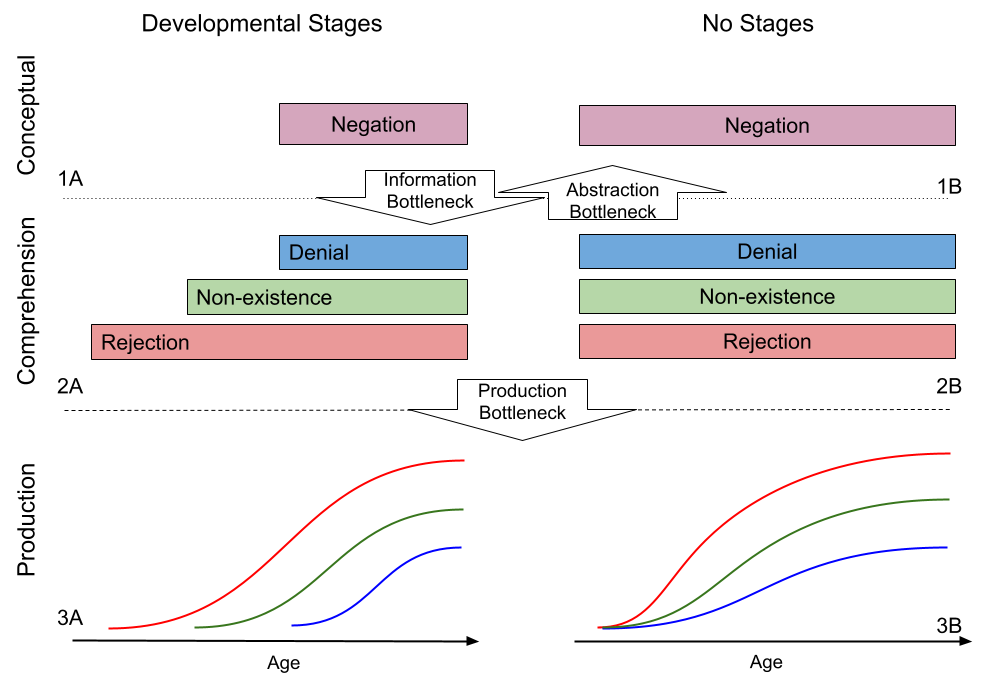
\includegraphics[width=1\linewidth]{pics/theory} \caption{Diagram of predictions for possible nativist and empiricist accounts for the development of negation in language production, language comprehension, and conceptual development.}\label{fig:theory}
\end{figure}

What are the predictions of empiricist and nativist approaches to logical concepts with respect to children's language development? Figure \ref{fig:theory} classifies possible predictions of these two approaches with respect to presence (A) or absence (B) of population-level stages in conceptual development (1), language comprehension (2), and language production (3). The two approaches differ fundamentally at the conceptual level: logical empiricism predicts the emergence of abstract negation (1A) while logical nativism considers it present from birth (1B). The classic empiricist account assumes that population-level conceptual development in stages is mirrored in both comprehension (2A) and production (3A). It proposes that children comprehend and produce communicative functions in fixed stages (e.g.~rejection followed by non-existence and denial). Only after learning these concrete instances of language use, do children abstract over them to extract negation as an abstract concept. This is why many studies in this tradition use the resence of stages in children's linguistic production as evidence for conceptual stages (Bloom, 1970; McNeill \& McNeill, 1968; Pea, 1978). The simplest nativist account does not predict any stages in comprehension (2B) or production (3B). It proposes that innate and abstract negation can be mapped to different communicative functions and be used in the right context. Analogous to classic logical empiricism, one might use the absence of stages in children's production as evidence for absence of conceptual stages and therefore logical nativism.

However, presence or absence of population-level stages in children's production does not necessitate presence of population-level stages in comprehension or conceptual development (McDermott-Hinman \& Feiman, In Press). The empiricist and nativist approaches can have more nuanced accounts. For example, it is possible for negation to be an innate abstract concept (1B) but due to insufficient linguistic and contextual information, certain communicative functions may be harder to comprehend and learn, resulting in population-level stages in comprehension (2A), and possibly production (2B). Following McDermott-Hinman and Feiman (In Press) we call this ``the information bottleneck''. A different version of this account may predict population-level stages in comprehension (2A) but not production (3B). A third nativist account may posit no information bottleneck and therefore no stages in comprehension (2B), but rather a production bottleneck that results in stages for language production (3A). Gomes et al. (2023) tested adults' ability to guess the presence or absence of negation in an utterance in child-directed speech and found that adults can more easily guess instances of prohibition than non-existence or denial with only video information and no linguistic context. Once the linguistic context was also provided, adults were more successful in guessing denial negation too. This study provides a proof of concept that an information bottleneck may cause population-level stages in comprehension of certain communicative functions, and possibly their production as well.

It is similarly possible to have different empiricist accounts (1A). For example, an empiricist account may predict population-level stages in comprehension (2A), yet no stages in production (3B), because of a ``production bottleneck'': by the time children start producing utterances the relevant conceptual development has already occurred and abstract negation is available for form-meaning mapping. Alternatively, a different empiricist account may posit no population-level stages for comprehension (i.e.~different children develop abstract negation using different communicative functions), yet predict population-level production stages (3A), again due to a production bottleneck: constructions that convey communicative functions may differ based on how hard or easy they are to produce. Finally a third empiricist approach may predict no population-level stages in either comprehension (2B) or production (3B). While children do develop negation by abstracting from concrete instances, they may do it in any order in comprehension or production. We can say the abstract category of negation develops later due to an ``abstraction bottleneck''.

Rejecting or corroborating each of these empiricist or nativist accounts require careful examination of the relevant facts in children's comprehension and production of linguistic neation, as well as their auxiliary ``bottleneck assumptions''. In this study, we use a relatively large collection of transcripts of parent-child interactions in English to investigate the development of seven negative constructions that typically convey seven communicative functions. For each negative construction, we both look at children's negative responses (saying \emph{no}) to parent utterances with that construction, as well as children's own productions of these constructions. Hence, our study examines the presence of stages in children's production in a direct way, and by using their one-word negative responses to parents utterances it also examines the presence of stages in their comprehension in an indirect way. We use growth curve analysis to model the development of each construction and assess their order of acquisition.

\section{Previous Studies}\label{previous-studies}

This section provides a relatively detailed review of previous literature on the development of negation in population-level stages. Those familiar with the literature can skip to Table \ref{tab:summary} and the few paragraphs after to recover the gist. Darwin (1872, Chapter 11) explained the emergence of linguistic negation using the function it plays in early communication. He hypothesized that nodding and shaking are the earliest expressions of affirmation and negation respectively: ``With infants, the first act of denial consists in refusing food; and I repeatedly noticed with my own infants, that they did so by withdrawing their heads laterally from the breast, or from anything offered them in a spoon \ldots{} {[}moreover{]} \ldots{} when the voice is exerted with closed teeth or lips, it produces the sound of the letter \emph{n} or \emph{m}. Hence we may account for the use of the particle \emph{ne} to signify negation, \ldots{}''. In later research, this communicative function of negation was referred to as ``rejection'' or ``refusal'' (Bloom, 1970; Choi, 1988; Pea, 1978).

Unlike Darwin, McNeill and McNeill (1968)'s developmental account did not start with rejection, but rather with expressing external states (non-existence of objects). They studied the development of three Japanese negative morphemes (\emph{nai}, \emph{iya}, \emph{iiya}) in the speech of a 27-month-old Japanese speaking girl called Izanami. According to McNeill and McNeill (1968), in Japanese, \emph{nai} expresses falsity of statements (e.g., ``no {[}that's not an apple{]}''), \emph{iya} expresses desires (e.g.,``no {[}I don't want an apple{]}''), and \emph{iiya} expresses contrast (e.g., ``no {[}I didn't have an apple. I had a pear{]}''). The appearance of these negative morphemes in the speech of a child reflects the developmental stages for the respective communicative functions. McNeill and McNeill (1968) reported that in the first stage, Izanami used a simple negation like \emph{nai} to express non-existence of events and objects. They also mentioned the early use of \emph{shira-nai} (``I don't know'') but did not incorporate it into their developmental account. In the second stage, Izanami used negation to mark incorrectness of statements, e.g., saying ``false''. Such use of negation was labeled as ``denials'' in later research. In stage three, negation was also used to express disapproval or rejection - like saying ``I don't want that''. In the fourth stage, Izanami used negation to express contrasts - as if to say ``not this but something else''. Finally in the last stage, Izanami had an abstract and multi-functional concept of negation. According to McNeill and McNeill (1968), these stages took about five months and started with expressing external states (non-existence of objects) before internal desires (rejection).

Bloom (1970) considered three communicative functions for early negation: non-existence, rejection, and denial. She studied three children, two from 19 months and another from 21 months of age. She argued that in all three children, negation was produced in the following order: non-existence, rejection, and denial. Table \ref{tab:bloom} provides a few examples for each category. Many of these examples do not immediately stand out as instances of their category. This is partly because many early examples in child production are fairly short with underspecified syntactic structures, leading their interpretations to be heavily reliant on the context. It is therefore hard to assess the intention behind the use of negation in such cases.

\begin{longtable}[]{@{}
  >{\raggedright\arraybackslash}p{(\columnwidth - 4\tabcolsep) * \real{0.4110}}
  >{\raggedright\arraybackslash}p{(\columnwidth - 4\tabcolsep) * \real{0.2877}}
  >{\raggedright\arraybackslash}p{(\columnwidth - 4\tabcolsep) * \real{0.3014}}@{}}
\caption{\label{tab:bloom} Examples of non-existence, rejection, and denial negation in the speech of Eric, Kathryn, and Gia from Bloom (1970).}\tabularnewline
\toprule\noalign{}
\begin{minipage}[b]{\linewidth}\raggedright
Non-existence
\end{minipage} & \begin{minipage}[b]{\linewidth}\raggedright
Rejection
\end{minipage} & \begin{minipage}[b]{\linewidth}\raggedright
Denial
\end{minipage} \\
\midrule\noalign{}
\endfirsthead
\toprule\noalign{}
\begin{minipage}[b]{\linewidth}\raggedright
Non-existence
\end{minipage} & \begin{minipage}[b]{\linewidth}\raggedright
Rejection
\end{minipage} & \begin{minipage}[b]{\linewidth}\raggedright
Denial
\end{minipage} \\
\midrule\noalign{}
\endhead
\bottomrule\noalign{}
\endlastfoot
\textbf{\emph{no}} \emph{more choochoo train} & \textbf{\emph{no}} \emph{train} & \textbf{\emph{no}} \emph{Daddy hungry} \\
\textbf{\emph{no}} \emph{more noise} & \textbf{\emph{no}} \emph{want this} & \textbf{\emph{no}} \emph{more birdie} \\
\textbf{\emph{no}} \emph{children} & \textbf{\emph{no}} \emph{bear book} & \textbf{\emph{no}} \emph{ready} \\
\textbf{\emph{no}} \emph{it won't fit} & \textbf{\emph{no}} \emph{go outside} & \textbf{\emph{no}} \emph{tire} \\
\emph{Kathryn} \textbf{\emph{no}} \emph{like celery} & \textbf{\emph{no}} \emph{dirty soap} & \textbf{\emph{no}} \emph{dirty} \\
\end{longtable}

Pea (1978) studied six children between the ages of 8-24 months. Children were recorded in their homes for about 90 minutes every month. All utterances that convey a negative meaning (e.g., containing \emph{no}, \emph{not}, \emph{all gone}, \emph{gone}, \emph{away}, \emph{stop}) and gestures (e.g., headshakes and headnods) were annotated and analyzed. Pea (1978) reported that children first started by using negation to express internal states (rejection), then external states (non-existence), and finally they used negation to connect language and the external world, (e.g., truth-functional negation or denials). This was in direct contradiction to McNeill and McNeill (1968) who proposed that children start with expressing external states before internal states.

de Villiers and de Villiers (1979) examined the communicative functions of negation in the speech of Adam (27-31 months), Eve (18-22 months), and their own child Nicholas (23-29 months). The first two children were recorded for an hour every two or three weeks (Brown, 1973). They annotated children's examples of negation for six communicative functions: non-existence, disappearance, non-occurrence, cessation, rejection, and denial. Disappearance referred to cases where an object became hidden and cessation referred to the use of negation when a movement or action stopped (e.g., ``no walk'' when a toy stopped walking). They found rejections and denials to be the most frequent (and most reliable-to-annotate) functions of negation, both present in the earliest samples of children's speech. The authors emphasized that there are considerable individual differences across the three children, whose production of negation mirror parent usage and child-directed speech; therefore the results cannot be taken as strong evidence that there are specific fixed stages of development for negation in child production.

Choi (1988) looked at the speech of 11 children (2 English, 4 Korean and 5 French speaking) between 19 to 40 months of age. She reported 9 communicative functions for children's negation shown in Table \ref{tab:choi}. She matched communicative functions with linguistic constructions that commonly convey them and proposed that these constructions and functions developed in three phases. First, children used \emph{no} alone to express the four functions of non-existence, prohibition, rejection, and failure. In the second phase, \emph{no} was used to express denial, inability, and epistemic negation. New constructions such as ``not+Noun Phrase'' (e.g., ``not a bee''), \emph{can't} (e.g.~``I can't put back''), and ``I don't know'' also emerged to express these functions. New constructions were also used to distinguish the functions in the previous phase such as rejection (e.g.~``I don't want to''). In the third phase, normative negation and inferential negation emerged in children's speech with modal auxiliaries like \emph{can't}. Negative forms for prohibition also appeared with the structure ``don't+Verb''.

\begin{longtable}[]{@{}
  >{\raggedright\arraybackslash}p{(\columnwidth - 6\tabcolsep) * \real{0.1944}}
  >{\raggedright\arraybackslash}p{(\columnwidth - 6\tabcolsep) * \real{0.2361}}
  >{\raggedright\arraybackslash}p{(\columnwidth - 6\tabcolsep) * \real{0.1944}}
  >{\raggedright\arraybackslash}p{(\columnwidth - 6\tabcolsep) * \real{0.3750}}@{}}
\caption{\label{tab:choi} Examples of communicative functions and their forms in Choi (1988).}\tabularnewline
\toprule\noalign{}
\begin{minipage}[b]{\linewidth}\raggedright
Function
\end{minipage} & \begin{minipage}[b]{\linewidth}\raggedright
Definition
\end{minipage} & \begin{minipage}[b]{\linewidth}\raggedright
Constructions
\end{minipage} & \begin{minipage}[b]{\linewidth}\raggedright
Example
\end{minipage} \\
\midrule\noalign{}
\endfirsthead
\toprule\noalign{}
\begin{minipage}[b]{\linewidth}\raggedright
Function
\end{minipage} & \begin{minipage}[b]{\linewidth}\raggedright
Definition
\end{minipage} & \begin{minipage}[b]{\linewidth}\raggedright
Constructions
\end{minipage} & \begin{minipage}[b]{\linewidth}\raggedright
Example
\end{minipage} \\
\midrule\noalign{}
\endhead
\bottomrule\noalign{}
\endlastfoot
Non-existence & expressing absence of entities & \emph{no}+V & ``no more'' (after emptying a bag) \\
Failure & expressing absence of an event & \emph{it won't} & ``not work'' (puzzle piece not fitting) \\
Prohibition & negating actions of others & \emph{don't} + V & \\
Rejection & negating the child's own actions & \emph{I don't want (to)} & \\
Denial & negating others' propositions & AUX + \emph{not} & ``no that's a pony'' (in response to ``Is this a car?'') \\
Inability & expressing physical inability & & ``can't!'' (taking two lego pieces apart) \\
Epistemic & lack of knowledge & \emph{I don't know} & ``I don't know'' (in response to ``what color is this?'') \\
Normative & expressing expected norms & \emph{(you) can't} & ``Him can't go on a boat'' \\
Inferential & child's inference about the listener & AUX + \emph{not} & ``I not broken this'' (seeing a broken crayon) \\
\end{longtable}

Cameron-Faulkner, Lieven, and Theakston (2007) recorded an English speaking child for an hour five times a week between the ages of 27 to 39 months. They classified his negative utterances into seven communicative functions by using categories from Choi (1988) and leaving out normative and inferential negation. They found examples of all seven functions in Brian's early speech. Starting at 27 months, single-word discourse-level \emph{no} was used to convey most functions but gradually other forms using \emph{not}, \emph{don't}, \emph{can't}, or \emph{won't} emerged and replaced \emph{no} in usage. For instance with inability and prohibition, Brian mostly used \emph{no} and \emph{not} at 27 months but switched to \emph{can't} to express inability, and \emph{don't} to express prohibition at 39 months. Cameron-Faulkner et al. (2007) argued that at 27 months, Brian had a broad conceptualization of negation and likely represented it as a ``unitary category in conceptual space''.

In a recent study, Nordmeyer and Frank (2018) looked at twice-a-month recordings of five children between the 12-36 months of age (1-3 years) in the Providence corpus (Demuth, Culbertson, \& Alter, 2006) and classified children's negative utterances into seven functional categories: disappearance, prohibition, self-prohibition, refusal (rejection), failure, denial, and unfulfilled expectations. Self-prohibition referred to cases where children addressed a prohibition to themselves (e.g.~saying \emph{no} to themselves when reaching for a forbidden object) and unfulfilled expectations referred to instances that expressed surprise when an object was not in an expected place, similar to some cases of non-existence in previous research. They found that refusal (rejections) and denial were the most common functions in children's production and that children varied with respect to which function was produced first. In line with de Villiers and de Villiers (1979), they concluded that the developmental trajectory of different communicative functions of negation may not be as consistent across individuals as some previous research had suggested.

\begin{longtable}[]{@{}
  >{\raggedright\arraybackslash}p{(\columnwidth - 6\tabcolsep) * \real{0.1644}}
  >{\raggedright\arraybackslash}p{(\columnwidth - 6\tabcolsep) * \real{0.1644}}
  >{\raggedright\arraybackslash}p{(\columnwidth - 6\tabcolsep) * \real{0.1644}}
  >{\raggedright\arraybackslash}p{(\columnwidth - 6\tabcolsep) * \real{0.5068}}@{}}
\caption{\label{tab:summary} Summary of previous studies on the development of negation's communicative functions; ``variable'' indicates the developmental order of different functions claimed by the study is not fixed.}\tabularnewline
\toprule\noalign{}
\begin{minipage}[b]{\linewidth}\raggedright
Study
\end{minipage} & \begin{minipage}[b]{\linewidth}\raggedright
Number of Children
\end{minipage} & \begin{minipage}[b]{\linewidth}\raggedright
Age Range (Months)
\end{minipage} & \begin{minipage}[b]{\linewidth}\raggedright
Proposed Functional Stages
\end{minipage} \\
\midrule\noalign{}
\endfirsthead
\toprule\noalign{}
\begin{minipage}[b]{\linewidth}\raggedright
Study
\end{minipage} & \begin{minipage}[b]{\linewidth}\raggedright
Number of Children
\end{minipage} & \begin{minipage}[b]{\linewidth}\raggedright
Age Range (Months)
\end{minipage} & \begin{minipage}[b]{\linewidth}\raggedright
Proposed Functional Stages
\end{minipage} \\
\midrule\noalign{}
\endhead
\bottomrule\noalign{}
\endlastfoot
McNeill and McNeill (1968) & 1 & 27-32 & non-existence \textgreater{} denial (non-contrastive) \textgreater{} rejection \textgreater{} denial (contrastive) \\
Bloom (1970) & 3 & 19-28 & non-existence \textgreater{} rejection \textgreater{} denial \\
Pea (1978) & 6 & 8-24 & rejection \textgreater{} non-existence \textgreater{} denial \\
de Villiers and de Villiers (1979) & 3 & 18-31 & rejection, denial (variable) \\
Choi (1988) & 11 & 19-40 & non-existence, prohibition, rejection, failure \textgreater{} denial, inability, epistemic \textgreater{} normative, inferential \\
Cameron-Faulkner et al. (2007) & 1 & 27-39 & non-existence, failure, prohibition, rejection, denial, inability, epistemic \\
Nordmeyer and Frank (2018) & 5 & 12-36 & denial, rejection, prohibition, failure, disappearance (variable) \\
\end{longtable}

Table \ref{tab:summary} provides a summary of previous research on the communicative functions of negation in children's speech. As the summary shows, there is currently no consensus on which functional categories should be included or in which order they are produced. Here we are going to discuss three possible reasons for this lack of consensus. First, de Villiers and de Villiers (1979) and Nordmeyer and Frank (2018) have emphasized that there is considerable variability among children and their parents in their use of negation. Given that previous studies have typically considered only a few children (3-4 on average), they could have reached conclusions that are true of their sample but not of the population of English-speaking children.

Second, previous studies have used monthly or fortnightly recordings of children's speech for about 60-90 minutes per recording session. Given that children produce many hours of speech daily, such sparse sampling might have created accidental gaps for certain communicative functions and consequently made it as if functions appear in ordered stages. The only study with relatively dense recording is Cameron-Faulkner et al. (2007) which reports the presence of all communicative functions in the child's speech from early on. However, the recordings for their study start at a later age (27 months) than many other studies.

Third, prior research shows that defining and detecting the communicative functions of negation is not a trivial task. Different studies have sometimes used different basic categories and different definitions or criteria for classifying negative utterances. Therefore, what counts as an instance of rejection or non-existence may vary among studies and contribute to the reported variability. Most importantly, annotations focus on many utterances with underspecified syntactic structures such as ``no car'' or ``no more'', which are highly ambiguous and can count as an instance of different communicative functions. Does ``no car'' mean ``there is no car here'' (non-existence) or ``I don't want a toy car'' (rejection)? Researchers often have to rely on the context but the context is not fully represented in many child language corpora used for annotations. More importantly, this approach is not scalable to larger numbers of children and bigger corpora since manual annotations take considerable amount of time, energy, and training. In the next section, we discuss how the current study addresses these three issues.

\section{Current Study}\label{current-study}

This study builds on previous research in four ways. First, it uses large corpora of parent-child interactions, aggregating speech samples from 693 children between the ages of 1-6 years (12-72 months). If the lack of consensus in previous research was mainly due to the small number of children or speech samples, increasing these numbers should address the issue. Aggregating speech samples across children would also provide denser samples at each age interval and reduce the possibility of accidental gaps. The reasoning behind this approach is that despite individual variation, if there are general developmental stages across children, they should be detectable in large aggregated corpora of children's speech.

Second, in this study we adopted Choi (1988)'s approach; instead of classifying negative communicative functions, we classified negative constructions that typically communicate those communicative functions (Table \ref{tab:summary}). Here by negative constructions, we refer to syntactic constructions modified by any one of the three negative morphemes in English: \emph{no}, \emph{not}, \emph{n't}. Table \ref{tab:constructions} summarizes the constructions in this study and the communicative functions they typically convey. We assume that communicative functions are defined at the level of pragmatics, and more specifically speech acts (J. L. Austin, 1975; Bach, 2006; Searle, 1979). Many factors come together to determine the communicative function of an utterance, including the semantics of the individual words, the way they are combined, the intonation, the common ground between discourse participants, the conversational context, etc. We do not assume that the negative constructions we define based on lexical and syntactic properties always convey the communicative function we have associated with them. In other words, constructions and communicative functions do not stand in a 1-1 relation. A construction can convey one or more communicative functions and vice versa. Nevertheless for our purposes, we only need a construction to ``typically'' convey a specific communicative function. For example, ``I don't know'' is typically and more often used to convey epistemic negation, even though it can also be used as a rejection from time to time.

If there are conceptual stages with downstream effects on comprehension and production of certain communicative functions as prior literature suggests, we should also see similar stages in children's comprehension and production of constructions that typically convey those communicative functions. Prior research has focused more on constructions with restricted form like \emph{no sound} that is quite ambiguous with respect to its communicative function The set of communicative functions we investigate in this study are not meant to be exhaustive or representative of all communicative functions of negation. We are simply testing the veracity the claim that communicative functions of negation develop in stages. T

This approach has several advantages, but also some disadvantages. Starting with the advantages, negative constructions are more concrete and thus easier to define than negative communicative functions. For example, utterances that combine negation with the main verb \emph{want} (e.g., ``I don't want that'') constitute a construction that typically conveys rejection. In addition, because of their concrete definitions, negative constructions can be detected and classified automatically in large corpora following lexical and syntactic heuristics. For instance, rather than manually annotating sentences that express rejection, it is relatively easier to automate the process by searching for utterances containing the verb \emph{want} modified by negative morphemes. However, using automated form-based annotations also comes with disadvantages. In manually annotating utterances, the annotator can potentially take into account factors other than the construction itself such as the conversational context, intonation, speaker intentions, etc. to determine the communicative function of the utterance. The automatic annotation we use here does not benefit from these other factors and therefore might miss the correct classification for some utterances. For example, as pointed out to us by an anonymous reviewer, the utterance ``I don't like that'' uses the construction that typically conveys ``rejection'', but can also be used to communicate ``prohibition'' (e.g.~imagine the child touching a forbidden object and the parent uses this utterance). The approach we have taken will not be sensitive to such pragmatically enriched cases. One can debate whether such uses truly count as a rejection (of an action performed by the addressee) or a prohibition (of the same action) as well, and indeed prior studies using human annotators often have to deal with criteria that settle such cases. If these cases constitute a majority of the uses for a particular construction, then using the construction as a proxy for communicative function would run into a serious problem. We do not have any evidence to suggest this is the case with the constructions we have in this study but encourage readers to keep this point as a caveat and limitation of this study in mind when considering the results and conclusions. More broadly, our approach is complementary to human annotation and should ideally converge in its conclusions with large scale human annotations.

\begin{longtable}[]{@{}
  >{\raggedright\arraybackslash}p{(\columnwidth - 4\tabcolsep) * \real{0.2222}}
  >{\raggedright\arraybackslash}p{(\columnwidth - 4\tabcolsep) * \real{0.2639}}
  >{\raggedright\arraybackslash}p{(\columnwidth - 4\tabcolsep) * \real{0.5139}}@{}}
\caption{\label{tab:constructions} Negative constructions used in this study that typically convey communicative functions studied in previous functional accounts of negation development.}\tabularnewline
\toprule\noalign{}
\begin{minipage}[b]{\linewidth}\raggedright
Function
\end{minipage} & \begin{minipage}[b]{\linewidth}\raggedright
Negative morpheme combines with
\end{minipage} & \begin{minipage}[b]{\linewidth}\raggedright
Examples (negative)
\end{minipage} \\
\midrule\noalign{}
\endfirsthead
\toprule\noalign{}
\begin{minipage}[b]{\linewidth}\raggedright
Function
\end{minipage} & \begin{minipage}[b]{\linewidth}\raggedright
Negative morpheme combines with
\end{minipage} & \begin{minipage}[b]{\linewidth}\raggedright
Examples (negative)
\end{minipage} \\
\midrule\noalign{}
\endhead
\bottomrule\noalign{}
\endlastfoot
Rejection & \emph{like}/\emph{want} & \emph{I} \textbf{\emph{not}} \emph{like it}; \textbf{\emph{not}} \emph{want it} \\
Non-existence & \emph{there}-expletive & \emph{there is} \textbf{\emph{no}} \emph{soup} \\
Prohibition & imperative subjectless \emph{do} & \emph{do} \textbf{\emph{not}} \emph{spill milk} \\
Inability & \emph{can} & \emph{I can} \textbf{\emph{not}} \emph{zip it} \\
Labeling (Denial) & nominal/adjectival predicates & \emph{that's} \textbf{\emph{not}} \emph{a crocodile}; \emph{it's} \textbf{\emph{no}} \emph{interesting} \\
Epistemic & \emph{know}/\emph{think}/\emph{remember} & \emph{I} \textbf{\emph{not}} \emph{know/think/remember} \\
Possession & \emph{have}/possesive pronouns & \textbf{\emph{not}} \emph{have the toy}; \textbf{\emph{not}} \emph{mine} \\
\end{longtable}

Third, focusing on children's productions runs the risk of underestimating their linguistic competence. Children produce shorter constructions and utterances before longer ones and typically develop the comprehension of those constructions before they can produce them (Clark, 2009). For example, children may be able to understand rejection and communicate it with a simple \emph{no} in response to a question like ``do you want an apple?'', before they can produce the full construction ``I don't want an apple''. In other words, the child may understand the meaning of the question as well as the meaning of \emph{no} and how it anaphorically negates the content of the previous utterance but due to production limitations not be able to produce the full sentence. In this study, we look at children's anaphoric negation with \emph{no} in response to parents positive constructions, as well as their productions of the corresponding negative constructions. We call the first ``discourse-level negation'' and the second ``sentence-level negation''. We take children's discourse-level negation as an approximation of their comprehension for negation and their sentence-level negation as an approximation for their production.

Fourth, we use growth curves to model the development of negative constructions in children's speech. We also estimate the age at which children reach maximum growth in their comprehension and production of different communicative functions of negation. For proxy measures of both comprehension and production, we check to see if the estimated age ranges support the hypothesis that negation develops in stages. We also ask whether developmental stages mirror each other in comprehension and production, or whether we find different stages and patterns of development for comprehension vs.~production.

\subsection{Methods}\label{methods}

We used the CHILDES database (MacWhinney, 2000)\footnote{Code and data are in quarantine at \url{https://thegoodplace.com}} and selected data of English speaking children with typical development within the age range of 12-72 months. Parents' and children's utterances were extracted via the childes-db (Sanchez et al., 2019) interface using the programming language R. In order to obtain (morpho)syntactic representations for parents' and children's utterances, we used the dependency grammar framework (Tesnière, 1959). Part-of-speech (POS) tags for each token within an utterance were automatically derived with Stanza (Qi, Zhang, Zhang, Bolton, \& Manning, 2020), an open-source natural language processing library; dependency relations for all utterances were acquired also in an automatic fashion using DiaParser (Attardi, Sartiano, \& Yu, n.d.), a dependency parsing system that has been demonstrated to achieve excellent performance for at least written texts in English.

At the sentence level, we characterized the syntactic features of the negative utterances associated with each communicative function (Table \ref{tab:constructions}), then classified utterances based on these features in a rule-based fashion with the help of POS information and syntactic dependencies. To decouple the development of the syntactic construction from the development of negation in that construction, we also examined the production of positive counterparts to each negative construction. The positive counterparts of our negative constructions share the same syntactic features (e.g., same head verb) but they have no negative morphemes (e.g.~``I know'' for ``I don't know''). Although these positive constructions do not express the same communicative function as their negative counterparts, our main purpose for including them is to factor in the development of the syntactic construction without negation as a reference.

At the discourse level, we analyze the negative constructions that the discourse particle \emph{no} stands for (or responds to in cases like prohibition, as discussed in the previous section). To achieve this, we selected utterances that started with negative discourse particles like ``no no I like it'' and the dependency parser had tagged their dependency relation as \emph{discourse}. We also included cases with repetitions of the discourse particle (``no no no''). For each negative utterance identified this way, we extracted the previous utterance (the antecedent) in the discourse context. For child speech, we included antecedents produced by either the parents or the children themselves. For parent speech, we only included interactions where the antecedent was produced by children. We then applied the same analyses performed on sentence level constructions to these antecedent utterances. The assumption is that the negative discourse particle \emph{no} is implicitly negating the content of the discourse antecedent.

We took age as a proxy for children's developmental stage and divided the 12-72 months range into monthly bins. We used the following two metrics to measure the production level of every communicative function at each age bin. First, we defined the ratio \(f_{c,t}\) for construction \(c\) and age bin \(t\) as the number of utterances in construction \(c\) and age bin \(t\) divided by the total number of utterances produced at age bin \(t\). For example, there are a total of 81,302 utterances produced by children at age 30 months in the data, out of which 391 were classified as rejections. Therefore the ratio of rejection at 30 months is 391/81,302 = 0.005.

\(f_{c, t} = \frac{n_{c,t}}{n_{t}}\)

Second, we borrowed the measure of ``cumulative (moving) ratio'' from the analysis of time series data (Wei, 2006). We defined the cumulative ratio \(F_{c,t}\) for a construction \(c\) at age bin \(t\), as the sum of the number of utterances produced with construction \(c\) from the first age bin to age bin \(t\), divided by the sum of all utterances produced between the first age bin and age bin \(t\). For instance, up to age 30 months, children in our corpus produced 721,748 total utterances, out of which 2,166 were instances of rejection. Therefore, the cumulative ratio of rejection at age 30 months is 2,166/721,748 = 0.003. Cumulative ratio provides a more smooth measure of children's production addressing data sparsity issues. It also provides fixed lower and upper bounds (no production and the total ratio of production) which fits the assumptions of our statistical modeling later. As far as we know, the conclusions of our study do not change if we use simple ratios instead of cumulative ratios.

Assuming that children accumulate linguistic knowledge throughout their development, this measure provides a more realistic and stable measure of children's productive capacity at each age.

\(F_{c, t} = \frac{\sum_{i=1}^{t} n_{c,i}}{\sum_{i=1}^{t} n_{i}}\)

The two ratios mentioned above were calculated for negative constructions (and their positive counterparts) at the sentence and discourse levels for children as well as parents. For the sake of presentations, our figures focus on the results of cumulative ratios. In addition, in this study we use parents' speech as a benchmark for children's development. Therefore, the subfigures within each figure contrast children's production to that of parents' at the corresponding age of the children.

\subsection{Results}\label{results}

In this section, we first present the results for each communicative function and its associated negative constructions separately, before aggregating and presenting them together. We start with rejections.

\subsubsection{Rejection}\label{rejection}

For instances of rejection and their positive counterparts, we selected utterances in which the lemma of the head verb of the phrase was either \emph{like} or \emph{want}. For negative instances, the head verb is modified by one of the three negative morphemes \emph{no}, \emph{not} or \emph{n't}, whereas cases including the same head verb but without negation were classified as positive (Table \ref{tab:rejection}). In particular, the negative utterances included cases in which the speakers describe their own desires with or without an auxiliary verb, examples that express rhetorical inquiries of desires from one interlocutor to another, and instances where the speaker is describing the desires of somebody else. Our search critiera for this function led to a total of 20,641 negative utterances (child: 9,398; parent: 11,243), and a total of 180,881 positive utterances (child: 63,427; parent: 117,454).

\begin{longtable}[]{@{}ll@{}}
\caption{\label{tab:rejection} Examples of sentence-level rejections and their positive counterparts in children's speech.}\tabularnewline
\toprule\noalign{}
Rejection (Negative) & Positive counterpart \\
\midrule\noalign{}
\endfirsthead
\toprule\noalign{}
Rejection (Negative) & Positive counterpart \\
\midrule\noalign{}
\endhead
\bottomrule\noalign{}
\endlastfoot
\emph{I} \textbf{\emph{no}} \emph{like sea} & \emph{she likes cheese} \\
\emph{do\textbf{n't}} \emph{wanna go} & \emph{I want it} \\
\emph{do\textbf{n't}} \emph{you wanna try it} & \emph{I wanna have that} \\
\emph{Sarah does\textbf{n't}} \emph{like that either} & \emph{she likes this one} \\
\end{longtable}

\begin{figure}[H]

{\centering 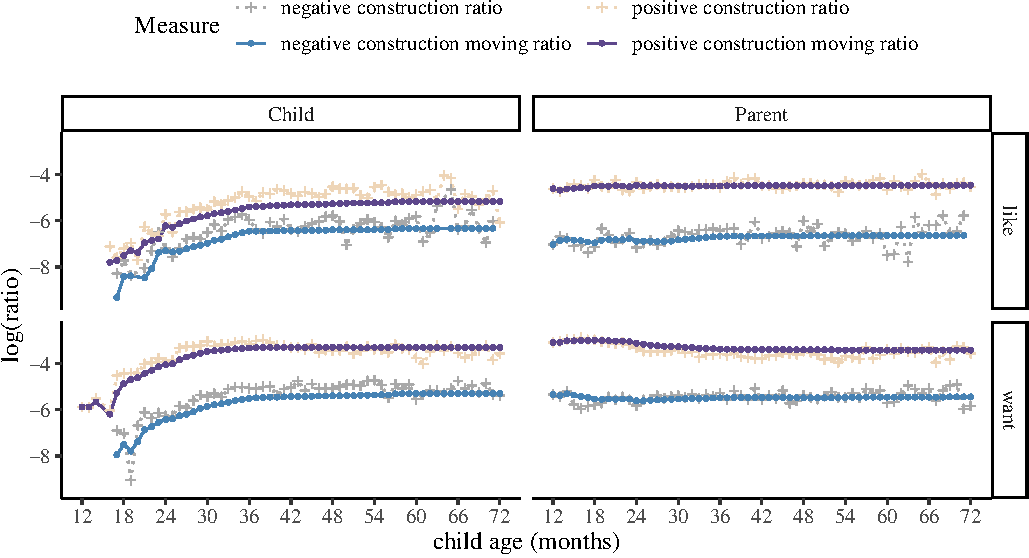
\includegraphics{neg_construction_article_files/figure-latex/emotion-1} 

}

\caption{Cumulative production ratios for the production of rejection at the sentence level for children between 12 to 72 months of age, and their parents. The y-axes are scaled differently for the panels to accommodate differences in production ratios.}\label{fig:emotion}
\end{figure}

Starting with our analysis at the sentence level, Figure \ref{fig:emotion} shows the cumulative ratios of parents' and children's instances of rejections and their positive counterparts (y-axis) with age along the x-axis. Overall, we see a similar pattern of production for rejection whether the head verb is \emph{want} or \emph{like} in child speech. Children's production of rejection gradually increases between the ages of 18 and 36 months. After about 36 months of age, children's production of these constructions starts to become relatively constant and close to parent levels. In all age bins, the production ratio for negative utterances was lower than that for their positive counterparts.

At the discourse level, we investigated discourse interactions (antecedent + utterance with negative discourse particle) in which the antecedent has one of the head verbs \emph{like} or \emph{want}, yet the head verb does not have to be modified by negative morphemes (Table \ref{tab:disreject}). We found a total of 1,329 such utterances (child: 680; parent: 649). As shown in Figure 2, children's production of \emph{no} to convey rejection increases regularly from the age of 18 - 36 months.\footnote{For each communicative function, at the discourse level we also examined cases of different subtypes (e.g., different head verbs) separately; though due to data sparsity issues, we collapsed these instances for our final analyses.} Overall, discourse-level rejection is produced more frequently in child speech compared to parent speech.

\begin{longtable}[]{@{}
  >{\raggedright\arraybackslash}p{(\columnwidth - 2\tabcolsep) * \real{0.4306}}
  >{\raggedright\arraybackslash}p{(\columnwidth - 2\tabcolsep) * \real{0.5694}}@{}}
\caption{\label{tab:disreject} Examples of discourse-level rejections in children's and parents' speech.}\tabularnewline
\toprule\noalign{}
\begin{minipage}[b]{\linewidth}\raggedright
Antecedent
\end{minipage} & \begin{minipage}[b]{\linewidth}\raggedright
Utterance
\end{minipage} \\
\midrule\noalign{}
\endfirsthead
\toprule\noalign{}
\begin{minipage}[b]{\linewidth}\raggedright
Antecedent
\end{minipage} & \begin{minipage}[b]{\linewidth}\raggedright
Utterance
\end{minipage} \\
\midrule\noalign{}
\endhead
\bottomrule\noalign{}
\endlastfoot
Parent: \emph{I want you to try it} & Child: \textbf{\emph{no no no}} \\
Parent: \emph{would you like to go} & Child: \textbf{\emph{no no}} \\
Child: \emph{I do\textbf{n't}} \emph{like that} & Parent: \textbf{\emph{no}} \emph{honey you have to try it} \\
Child: \emph{I want it} & Parent: \textbf{\emph{no}} \emph{this is not for you} \\
\end{longtable}

\begin{figure}[H]

{\centering 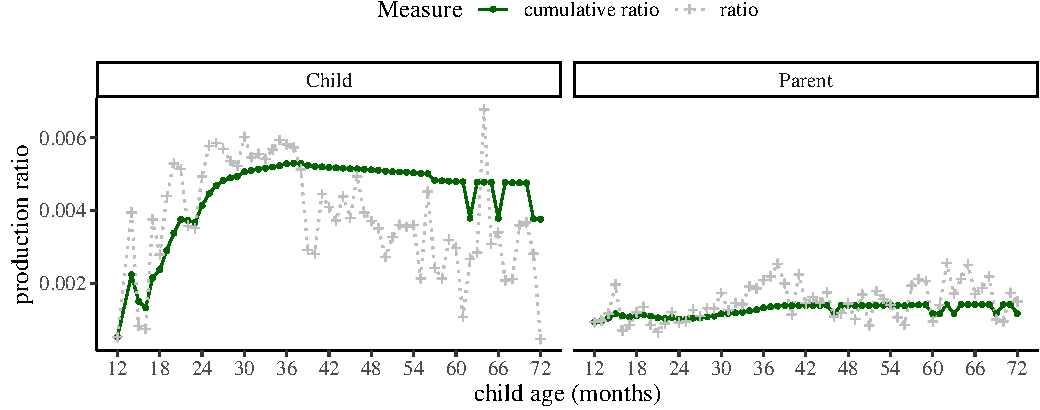
\includegraphics{neg_construction_article_files/figure-latex/emotiondiscourse-1} 

}

\caption{Cumulative production ratios for the production of rejection at the discourse level for children between 12 to 72 months of age, and their parents.}\label{fig:emotiondiscourse}
\end{figure}

\subsubsection{Non-existence}\label{non-existence}

For the function of non-existence, we searched for the English expletive construction and extracted utterances that had \emph{there}-expletives, followed by a copula, and a noun phrase (phrases headed by either nouns or pronouns). We classified utterances where the predicate was modified by negation as negative, and the rest as positive. This led to a total of 1,983 negative utterances (child: 498; parent: 1,485), and 35,287 positive utterances (child: 8,385; parent: 26,902).

\begin{longtable}[]{@{}ll@{}}
\caption{\label{tab:nonexist} Examples of sentence-level non-existence and positive counterparts in children's speech.}\tabularnewline
\toprule\noalign{}
Non-existence (Negative) & Positive counterpart \\
\midrule\noalign{}
\endfirsthead
\toprule\noalign{}
Non-existence (Negative) & Positive counterpart \\
\midrule\noalign{}
\endhead
\bottomrule\noalign{}
\endlastfoot
\emph{there's} \textbf{\emph{no}} \emph{(more) water} & \emph{there are books} \\
\emph{there is} \textbf{n't} \emph{it} & \emph{there is it} \\
\emph{there's} \textbf{\emph{no}} \emph{more cheese} & \emph{there is the toy} \\
\emph{there is} \textbf{\emph{no}} \emph{food} & \emph{there is an apple} \\
\end{longtable}

At the sentence level, children produce negative constructions to express non-existence less frequently than they do for the positive counterparts. As presented in Figure \ref{fig:existence}, the cumulative ratio for the production of non-existence increases mostly from 18 to 36 months. Then around and after 36 months of age, children's production gradually reaches a stable ratio but stays below parents' level. Notice that there appears to be slight fluctuations of cumulative ratios between the age of 19 and 25 months in child speech. A closer inspection of the data reveals that within that age range, the frequency of negative utterances at most ages is either one or zero. Therefore as the number of total utterances increases along the developmental trajectory, the cumulative ratio for non-existence utterances actually decreases in this brief period.

\begin{figure}[H]

{\centering 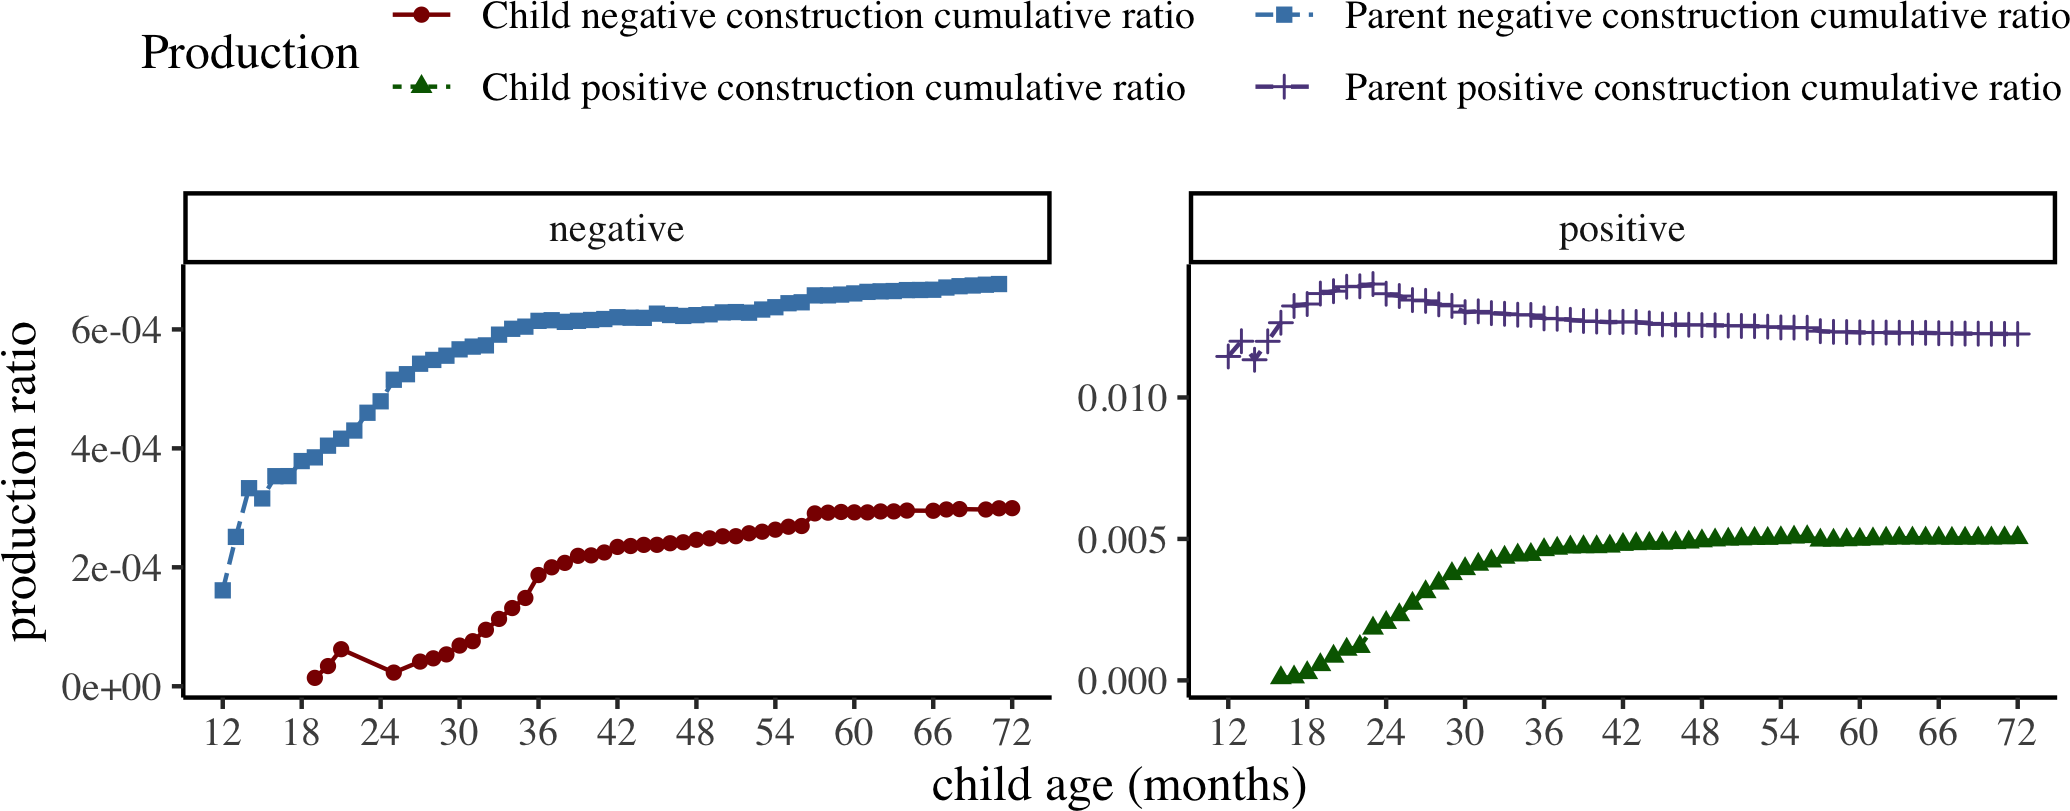
\includegraphics{neg_construction_article_files/figure-latex/existence-1} 

}

\caption{Cumulative production ratios for the production of non-existence at the sentence level for children between 12 to 72 months of age, and their parents. The y-axes are scaled differently for the panels to accommodate differences in production ratios.}\label{fig:existence}
\end{figure}

For non-existence at the discourse level, we applied similar selection criteria and extracted utterances (negative and positive) with existential constructions in their antecedents (Table \ref{tab:disexist}). This led to a total of 118 utterances (child: 63; parent: 55). As Figure \ref{fig:existencediscourse} shows, there is an increase in children's responses with \emph{no} to parents' existential utterances between the ages of 18 and 36 months. After 36 months, despite the fact that ratios show fluctuations, the cumulative ratios of children's production seem stable and similar. Therefore with non-existence, both sentence-level and discourse level analyses point to substantial development in the age rage of 18-36 months.

\begin{longtable}[]{@{}ll@{}}
\caption{\label{tab:disexist} Examples of discourse-level non-existence in children's and parents' speech.}\tabularnewline
\toprule\noalign{}
Antecedent & Utterance \\
\midrule\noalign{}
\endfirsthead
\toprule\noalign{}
Antecedent & Utterance \\
\midrule\noalign{}
\endhead
\bottomrule\noalign{}
\endlastfoot
Parent: \emph{is there a bunny} & Child: \textbf{\emph{no no}} \emph{bunny} \\
Parent: \emph{is there a table} & Child: \textbf{\emph{no no}} \\
Child: \emph{there is my ball} & Parent: \textbf{\emph{no}} \emph{that's not yours} \\
Child: \emph{is there lunch bag} & Parent: \textbf{\emph{no}} \emph{not yet sweety} \\
\end{longtable}

\begin{figure}[H]

{\centering 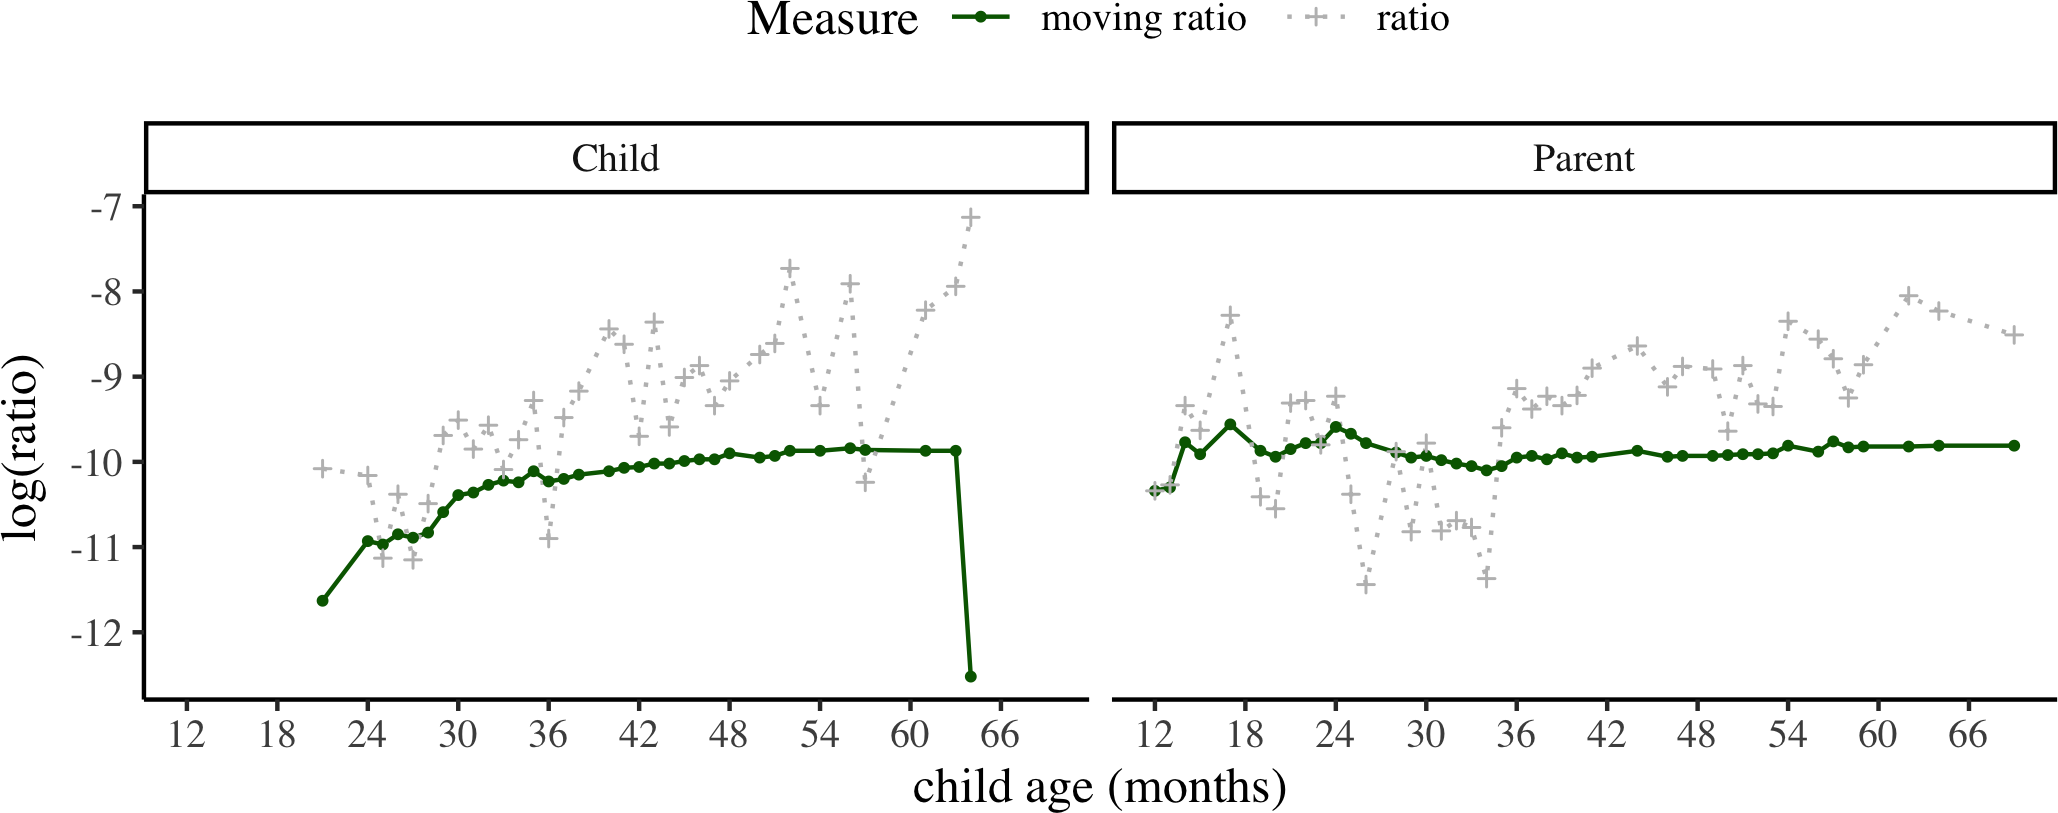
\includegraphics{neg_construction_article_files/figure-latex/existencediscourse-1} 

}

\caption{Cumulative production ratios for the production of non-existence at the discourse level for children between 12 to 72 months of age, and their parents.}\label{fig:existencediscourse}
\end{figure}

\subsubsection{Prohibition}\label{prohibition}

For constructions that typically convey prohibition, we extracted utterances that were labeled as ``imperatives'' in the CHILDES database. In particular, we selected instances where the head verbs do not take any subjects. As before, cases without any negative morphemes are considered as positive. For negative constructions, we chose structures where the negative morphemes are combined with the auxiliary verb \emph{do} and they together modify the head verbs of the sentences. In order to not have overlap with rejection, non-existence, epistemic negation and possession (see below), our search excluded utterances where the head verb had any of the following lemma forms: \emph{like}, \emph{want}, \emph{know}, \emph{think}, \emph{remember}, \emph{have}. This resulted in a total of 1,056 negative utterances (child: 303; parent: 753), and 25,542 positive utterances (child: 8,659; parent: 16,883).

Figure \ref{fig:prohibition} demonstrates the cumulative ratios of prohibition and their positive counterparts in parents' and children's production at the sentence level. In both child and parent speech, negative constructions for prohibition are consistently produced less frequently than their positive counterparts. Children produce negative imperatives more and more often between 24 and 36 months. In comparison, the cumulative ratio in parent speech gradually decreases at the beginning when children are between 12 - 24 months. Yet overall, children's production remains consistently lower than parents' production of prohibition. This might be due to the social nature of parent-child interactions, in which it is more likely for parents to explicitly command and direct children's actions than the other way round.

\begin{longtable}[]{@{}ll@{}}
\caption{\label{tab:prohibit} Examples of sentence-level prohibition and positive counterparts in children's speech.}\tabularnewline
\toprule\noalign{}
Prohibition (Negative) & Positive counterpart \\
\midrule\noalign{}
\endfirsthead
\toprule\noalign{}
Prohibition (Negative) & Positive counterpart \\
\midrule\noalign{}
\endhead
\bottomrule\noalign{}
\endlastfoot
\emph{do} \textbf{n't} \emph{blame Charlotte} & \emph{cook it} \\
\emph{do} \textbf{n't} \emph{do that} & \emph{try this} \\
\emph{do} \textbf{\emph{not}} \emph{touch that} & \emph{drink your water} \\
\emph{do} \textbf{\emph{not}} \emph{break it} & \emph{come here} \\
\end{longtable}

\begin{figure}[H]

{\centering 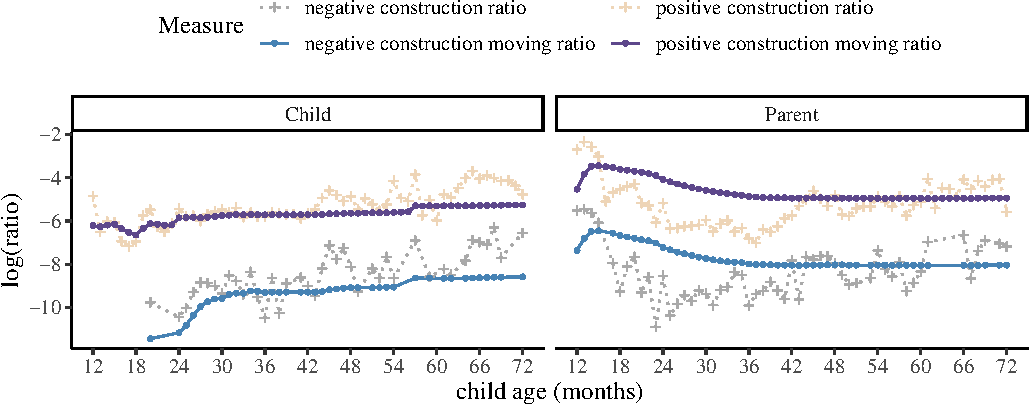
\includegraphics{neg_construction_article_files/figure-latex/prohibition-1} 

}

\caption{Cumulative production ratios for the production of prohibition at the sentence level for children between 12 to 72 months of age, and their parents. The y-axes are scaled differently for the panels to accommodate differences in production ratios.}\label{fig:prohibition}
\end{figure}

At the discourse level, we selected utterances where \emph{no} serves as a discourse response particle to antecedents that were subjectless imperatives headed by a verb. Again we excluded cases where the head verbs have any of the following lemmas: \emph{like}, \emph{want}, \emph{know}, \emph{think}, \emph{remember}, and \emph{have}. We would like to point out that in these instances, children's (and parents') production of \emph{no} is not necessarily negating the content of the antecedent prohibition. Instead we simply included these cases as a way of probing children's negative responses to imperatives, and also to be consistent with our analyses of the negative constructions of other communicative functions. Our search resulted in a total of 8 utterances (child: 4; parent: 4). As shown in Figure \ref{fig:prohibitiondiscourse}, both children's and parents' usage of negation as a response particle to imperatives gradually decrease before 36 months, then stays relatively stable after. Nevertheless, given the extremely small sample size here, these observations are not conclusive.

\begin{longtable}[]{@{}
  >{\raggedright\arraybackslash}p{(\columnwidth - 2\tabcolsep) * \real{0.4861}}
  >{\raggedright\arraybackslash}p{(\columnwidth - 2\tabcolsep) * \real{0.5139}}@{}}
\caption{\label{tab:disprohib} Examples of discourse-level prohibition in children's and parents' speech.}\tabularnewline
\toprule\noalign{}
\begin{minipage}[b]{\linewidth}\raggedright
Antecedent
\end{minipage} & \begin{minipage}[b]{\linewidth}\raggedright
Utterance
\end{minipage} \\
\midrule\noalign{}
\endfirsthead
\toprule\noalign{}
\begin{minipage}[b]{\linewidth}\raggedright
Antecedent
\end{minipage} & \begin{minipage}[b]{\linewidth}\raggedright
Utterance
\end{minipage} \\
\midrule\noalign{}
\endhead
\bottomrule\noalign{}
\endlastfoot
Parent: \emph{put away your toys} & Child: \textbf{\emph{no}} \emph{mommy I like these} \\
Parent: \emph{do\textbf{n't}} \emph{put it there} & Child: \textbf{\emph{no}} \emph{I really want to} \\
Child: \emph{give it to me} & Parent: \textbf{\emph{no}} \emph{not right now} \\
Child: \emph{try it} & Parent: \textbf{\emph{no no}} \emph{please} \\
\end{longtable}

\begin{figure}[H]

{\centering 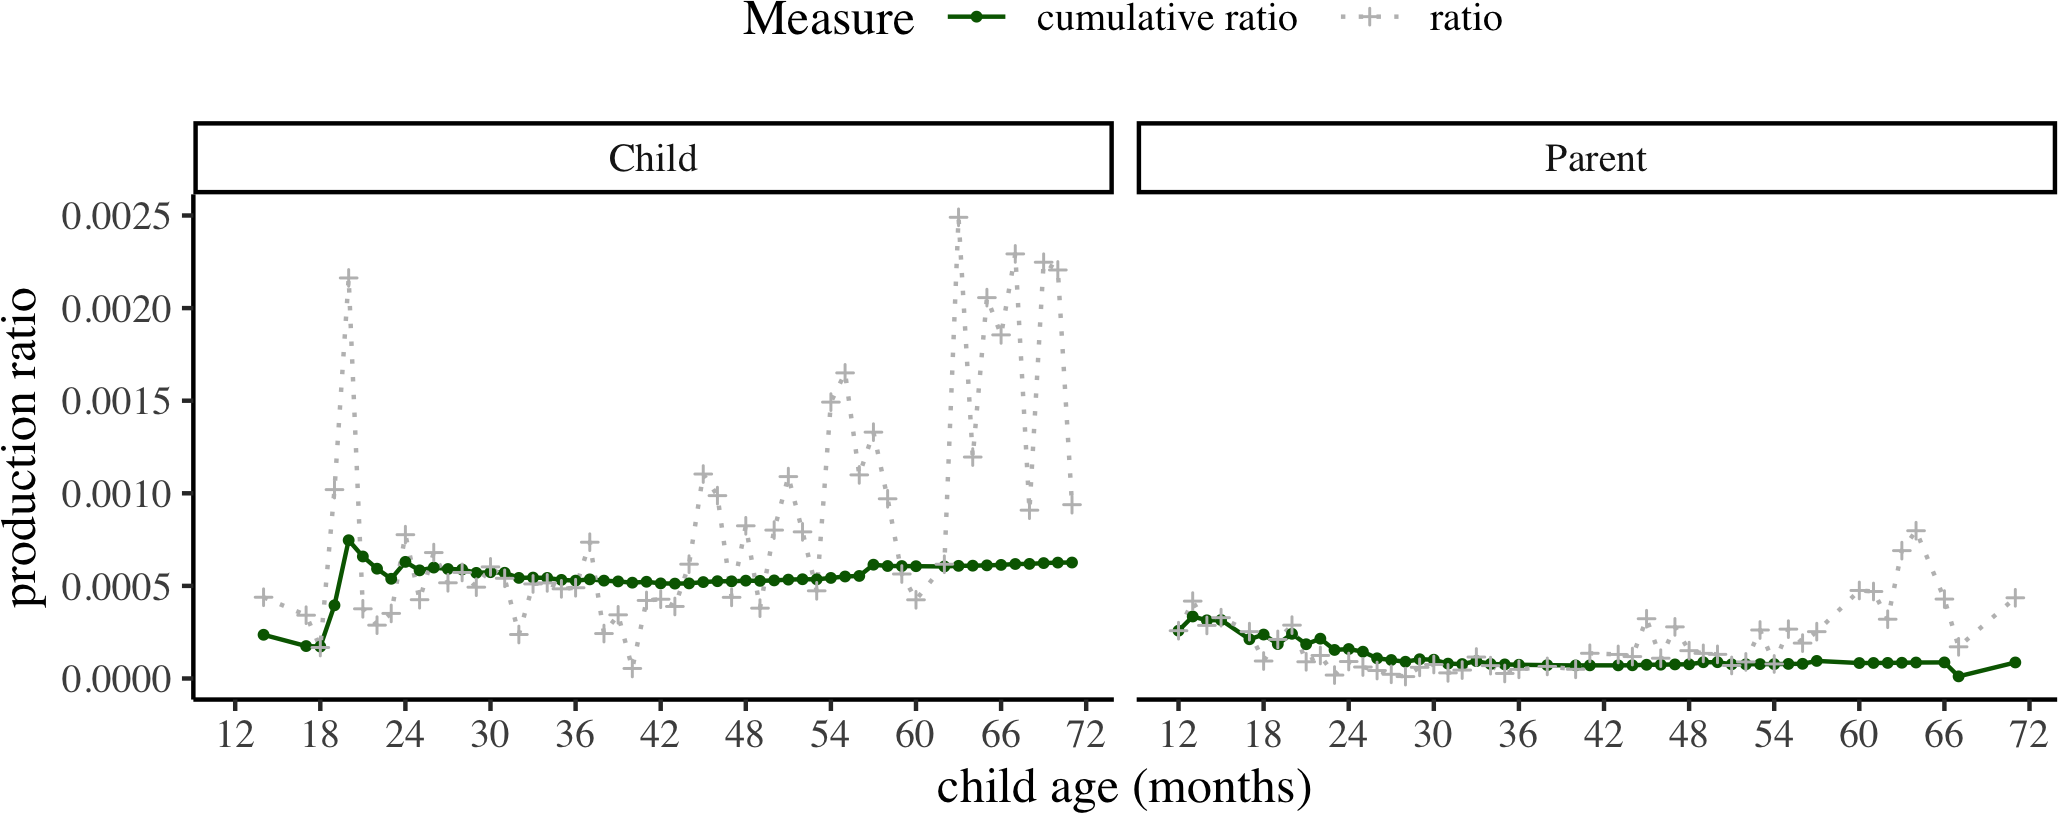
\includegraphics{neg_construction_article_files/figure-latex/prohibitiondiscourse-1} 

}

\caption{Cumulative production ratios for the production of prohibition at the discourse level for children between 12 to 72 months of age, and their parents.}\label{fig:prohibitiondiscourse}
\end{figure}

\subsubsection{Inability}\label{inability}

For the function of inability, we analyzed instances with head verbs that are modified by the modal auxiliaries \emph{can} and \emph{could}. If the head verb was also modified by a negative morpheme, we classified it as negative. Otherwise, we considered it positive. Depending on the larger context, the interpretation of utterances such as ``can't go yet'' and ``this can't go in the box'' could be deontic (e.g., ``not allowed to go yet''). Given the automatic fashion of our approach, in order to limit the number of cases that potentially yield readings other than (in)ability, we excluded cases without a subject or with subjects that were not first person singular \emph{I}. This led to 7,115 negative utterances (child: 3,917; parent: 3,198), and 14,433 positive utterances (child: 7,589; parent: 6,844). Table \ref{tab:inab} shows a few example of the cases we considered.

\begin{longtable}[]{@{}ll@{}}
\caption{\label{tab:inab} Examples of sentence-level inability and positive counterparts in children's speech.}\tabularnewline
\toprule\noalign{}
Inability (Negative) & Positive counterpart \\
\midrule\noalign{}
\endfirsthead
\toprule\noalign{}
Inability (Negative) & Positive counterpart \\
\midrule\noalign{}
\endhead
\bottomrule\noalign{}
\endlastfoot
\emph{I ca\textbf{n't}} \emph{see} & \emph{I could do it} \\
\emph{I ca\textbf{n't}} \emph{go} & \emph{I could help it} \\
\emph{I can} \textbf{\emph{not}} & \emph{I can try} \\
\emph{I can} \textbf{\emph{not}} \emph{do it} & \emph{I can put it back} \\
\end{longtable}

Figure \ref{fig:inability} shows cumulative ratios of parents' and children's production of constructions that convey (in)ability. Similar to previous constructions, positive instances are generally more frequent than negative ones. Children produce inability more and more frequently between 18-36 months. After 36 months, their production is gradually becoming stable and higher than parents' production level.

\begin{figure}[H]

{\centering 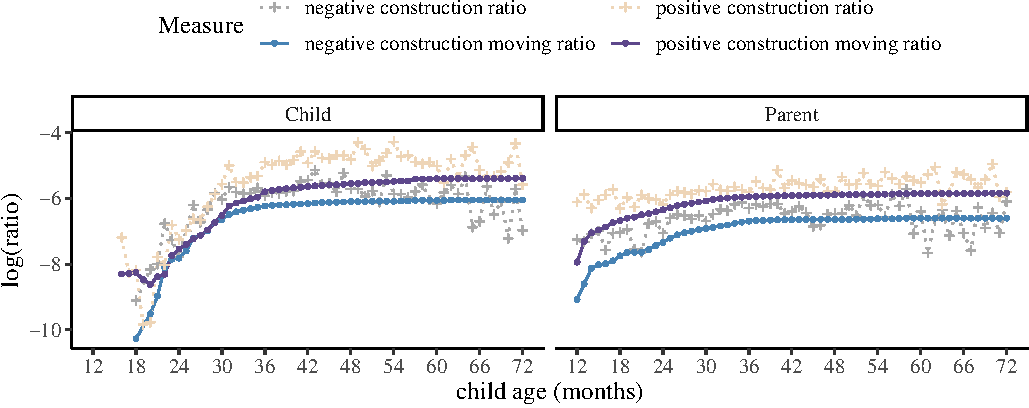
\includegraphics{neg_construction_article_files/figure-latex/inability-1} 

}

\caption{Cumulative production ratios for the production of inability at the sentence level for children between 12 to 72 months of age, and their parents. The y-axes are scaled differently for the panels to accommodate differences in production ratios.}\label{fig:inability}
\end{figure}

\begin{longtable}[]{@{}ll@{}}
\caption{\label{tab:disinability} Examples of discourse level inability in children's and parents' speech.}\tabularnewline
\toprule\noalign{}
Antecedent & Utterance \\
\midrule\noalign{}
\endfirsthead
\toprule\noalign{}
Antecedent & Utterance \\
\midrule\noalign{}
\endhead
\bottomrule\noalign{}
\endlastfoot
Parent: \emph{I can do it for you} & Child: \textbf{\emph{no no}} \\
Parent: \emph{I ca\textbf{n't}} \emph{see} & Child: \textbf{\emph{no}} \emph{try again} \\
Child: \emph{I can pour this} & Parent: \textbf{\emph{no no}} \emph{please} \\
Child: \emph{I ca\textbf{n't}} \emph{finish} & Parent: \textbf{\emph{no}} \emph{you have to} \\
\end{longtable}

At the discourse level, we chose utterances with the negative particle \emph{no} in response to antecedents that had a similar structure to the inability construction defined at the sentence level. In these interactions, \emph{no} is not always negating the content of the antecedents exactly. However, similar to our motivation for analyzing prohibition at the discourse level, we included these instances to investigate children's (and parents') negative responses to (in)ability more broadly. This yielded a total of 179 negative utterances (child: 58; parent: 121). Figure \ref{fig:inabilitydiscourse} presents the cumulative ratios for parents' and children's production of discourse-level inability. Children's production gradually increases from 24 to 36 months and stabilizes after 36 months at a similar rate to that of parent's. Children may be producing instances of inability more than parents because due to their developmental limitations they have more reason to express inability, and perhaps seek help.

\begin{figure}[H]

{\centering 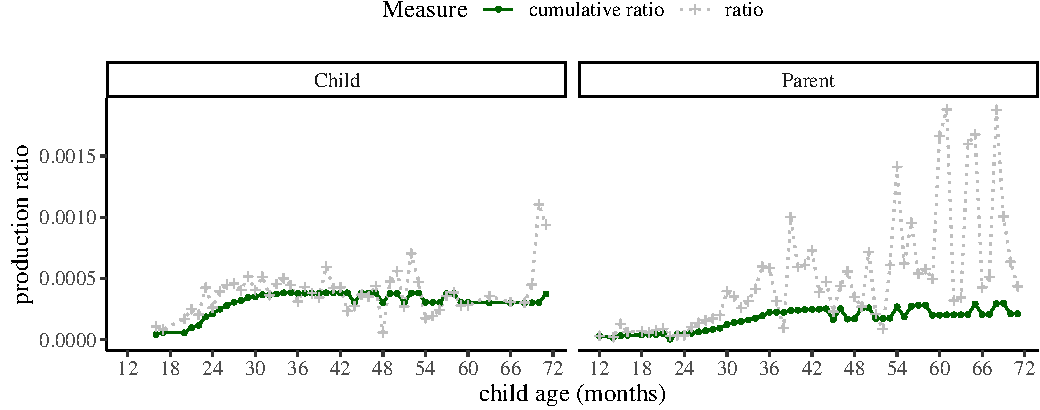
\includegraphics{neg_construction_article_files/figure-latex/inabilitydiscourse-1} 

}

\caption{Cumulative production ratios for the production of inability at the discourse level for children between 12 to 72 months of age, and their parents.}\label{fig:inabilitydiscourse}
\end{figure}

\subsubsection{Labeling}\label{labeling}

To capture the function of labeling at the sentence level, we concentrated on copula structures in which the predicate is a nominal or an adjectival phrase. Specifically, the nominal predicates exclude possessive pronouns (e.g., ``mine'') as well as nominals with a possessive dependent (e.g., ``my book'') in order to not overlap with the communicative function of possession (see Possession below). We considered instances where the predicate is modified by negative morphemes as negative, and others as positive. To also avoid overlap with cases of non-existence, none of the utterances contained expletives (e.g., ``there is no book''). This resulted in a total of 36,410 negative utterances (Child: 6,193; Parent: 30,217), and 484,679 positive utterances (Child: 121,107; Parent: 363,572). It is important to note that ``labeling'' as a communicative function can be considered as a subset of what is called ``denial'' in prior literature.

\begin{longtable}[]{@{}ll@{}}
\caption{\label{tab:label} Examples of sentence-level labeling (negative) and positive counterparts in children's speech.}\tabularnewline
\toprule\noalign{}
Labeling (Negative) & Positive counterpart \\
\midrule\noalign{}
\endfirsthead
\toprule\noalign{}
Labeling (Negative) & Positive counterpart \\
\midrule\noalign{}
\endhead
\bottomrule\noalign{}
\endlastfoot
\emph{that's not a farmer} & \emph{this is a book} \\
\emph{this is not the book} & \emph{this is nice} \\
\emph{I'm not a heavy baby Mum} & \emph{it's a nice bowl} \\
\emph{It's no good} & \emph{she's pretty} \\
\end{longtable}

Figure \ref{fig:learning} shows cumulative ratios for parent's and children's production of the labeling construction at the sentence level. In both parent and children speech, the frequency of positive counterparts is consistently higher than that of negative labeling instances. Children's production of negative labeling increases between 18-36 months, and remains stable after then; though the production ratios remained lower than those of parents'.

\begin{figure}[H]

{\centering 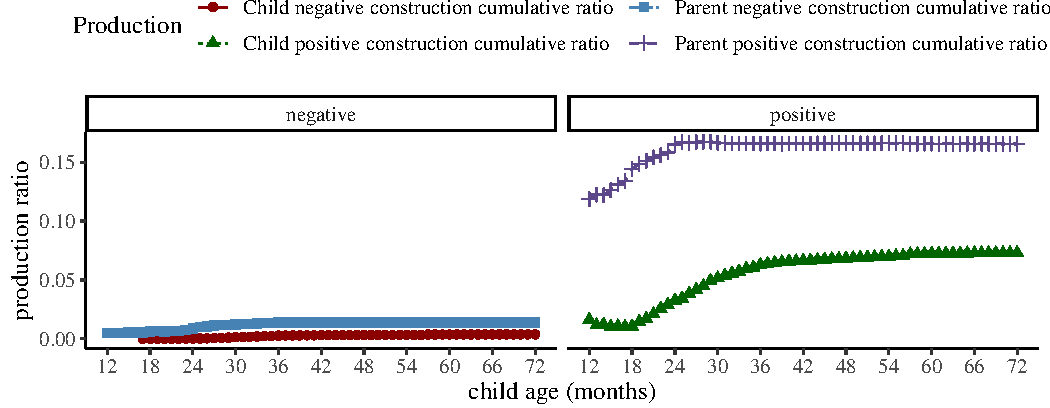
\includegraphics{neg_construction_article_files/figure-latex/learning-1} 

}

\caption{Cumulative production ratios for the production of (negative) labeling at the sentence level for children between 12 to 72 months of age, and their parents. The y-axes are scaled differently for the panels to accommodate differences in production ratios.}\label{fig:learning}
\end{figure}

At the discourse level, we selected antecedent utterances with copula structures that are combined with a nominal or an adjectival predicate (\ref{tab:dislabel}). In total we found 2,232 utterances (Child: 1,448; Parent: 784). The cumulative ratios for labeling instances at the discourse level are illustrated in Figure \ref{fig:learningdiscourse}. There is an increase in children's use of \emph{no} to negate labeling between 18 to 36 months. After 36 months, however, the production stays at a stable rate above parents level.

\begin{longtable}[]{@{}ll@{}}
\caption{\label{tab:dislabel} Examples of discourse-level labeling (negative) in children's and parents' speech.}\tabularnewline
\toprule\noalign{}
Antecedent & Utterance \\
\midrule\noalign{}
\endfirsthead
\toprule\noalign{}
Antecedent & Utterance \\
\midrule\noalign{}
\endhead
\bottomrule\noalign{}
\endlastfoot
Parent: \emph{is this one good} & Child: \textbf{\emph{no}} \emph{it's not} \\
Parent: \emph{are you a captain} & Child: \textbf{\emph{no}} \emph{I'm not} \\
Child: \emph{that's the one} & Parent: \textbf{\emph{no}} \emph{it's the green one} \\
Child: \emph{this is the key} & Parent: \textbf{\emph{no no}} \\
\end{longtable}

\begin{figure}[H]

{\centering 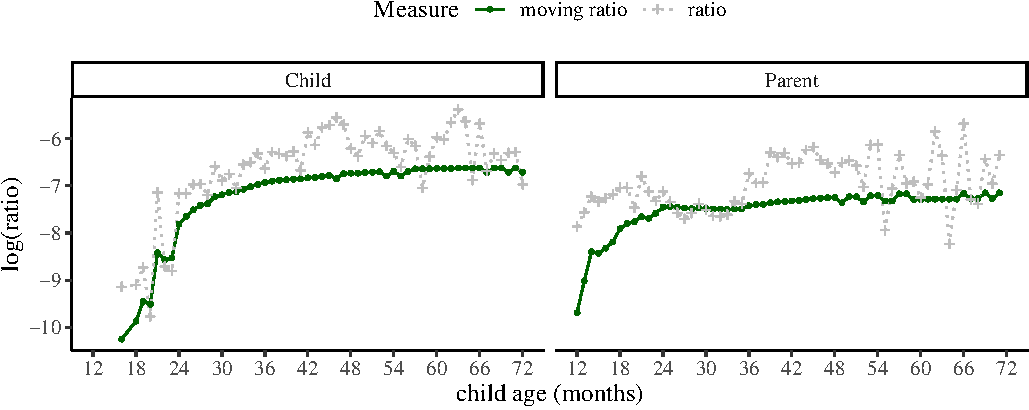
\includegraphics{neg_construction_article_files/figure-latex/learningdiscourse-1} 

}

\caption{Cumulative production ratios for the production of (negative) labeling at the discourse level for children between 12 to 72 months of age, and their parents.}\label{fig:learningdiscourse}
\end{figure}

\subsubsection{Epistemic Negation}\label{epistemic-negation}

Previous studies have reported instances in which children combined negative morphemes with mental state verbs such as \emph{know}, \emph{think}, and \emph{remember} to express ``epistemic negation'' (Choi, 1988). To define epistemic constructions, we also focused on these three verbs. For sentence-level epistemic negation, we analyzed negative utterances where these verbs were modified by negative morphemes, possibly after combining with an auxiliary verb like \emph{do}. Table \ref{tab:epistem} shows a few examples. Instances where the speaker asked about or described the negative epistemic state of another speaker were also included, leading to 31,696 negative utterances in total (child: 9,852; parent: 21,844). For the positive counterparts, we selected instances with the same head verbs except that these verbs were not modified by negation. This resulted in a total of 95,679 positive utterances (child: 16,322; parent: 79,357).

\begin{longtable}[]{@{}ll@{}}
\caption{\label{tab:epistem} Examples of sentence-level epistemic negation and positive counterparts in children's speech.}\tabularnewline
\toprule\noalign{}
Epistemic (Negative) & Positive counterpart \\
\midrule\noalign{}
\endfirsthead
\toprule\noalign{}
Epistemic (Negative) & Positive counterpart \\
\midrule\noalign{}
\endhead
\bottomrule\noalign{}
\endlastfoot
\emph{I} \textbf{\emph{not}} \emph{know} & \emph{I know} \\
\emph{I did\textbf{n't}} \emph{remember} & \emph{she remembers} \\
\emph{I do\textbf{n't}} \emph{think so} & \emph{he thinks this one is good} \\
\emph{She does\textbf{n't}} \emph{know this} & \emph{She knows about this} \\
\end{longtable}

Figure \ref{fig:epistemic} shows the cumulative ratios of the epistemic construction as defined above in parents' and children's speech at the sentence level. Across the three head verbs, children's production increases substantially from 18 to 36 months then gradually becomes stable yet still lower than parents' production level afterwards. The number of epistemic instances headed by \emph{know} is overall higher than the number of cases headed by either \emph{remember} or \emph{think}, an observation that is consistent in both negative constructions and positive counterparts. However, the majority of negative constructions headed by \emph{know} are idiomatic expressions such as ``I don't know'' (51.66\%) or ``don't know'' (13.73\%). Positive epistemic utterances are in general more frequent than negative ones, with the exception of \emph{know} in child speech.

\begin{figure}[H]

{\centering 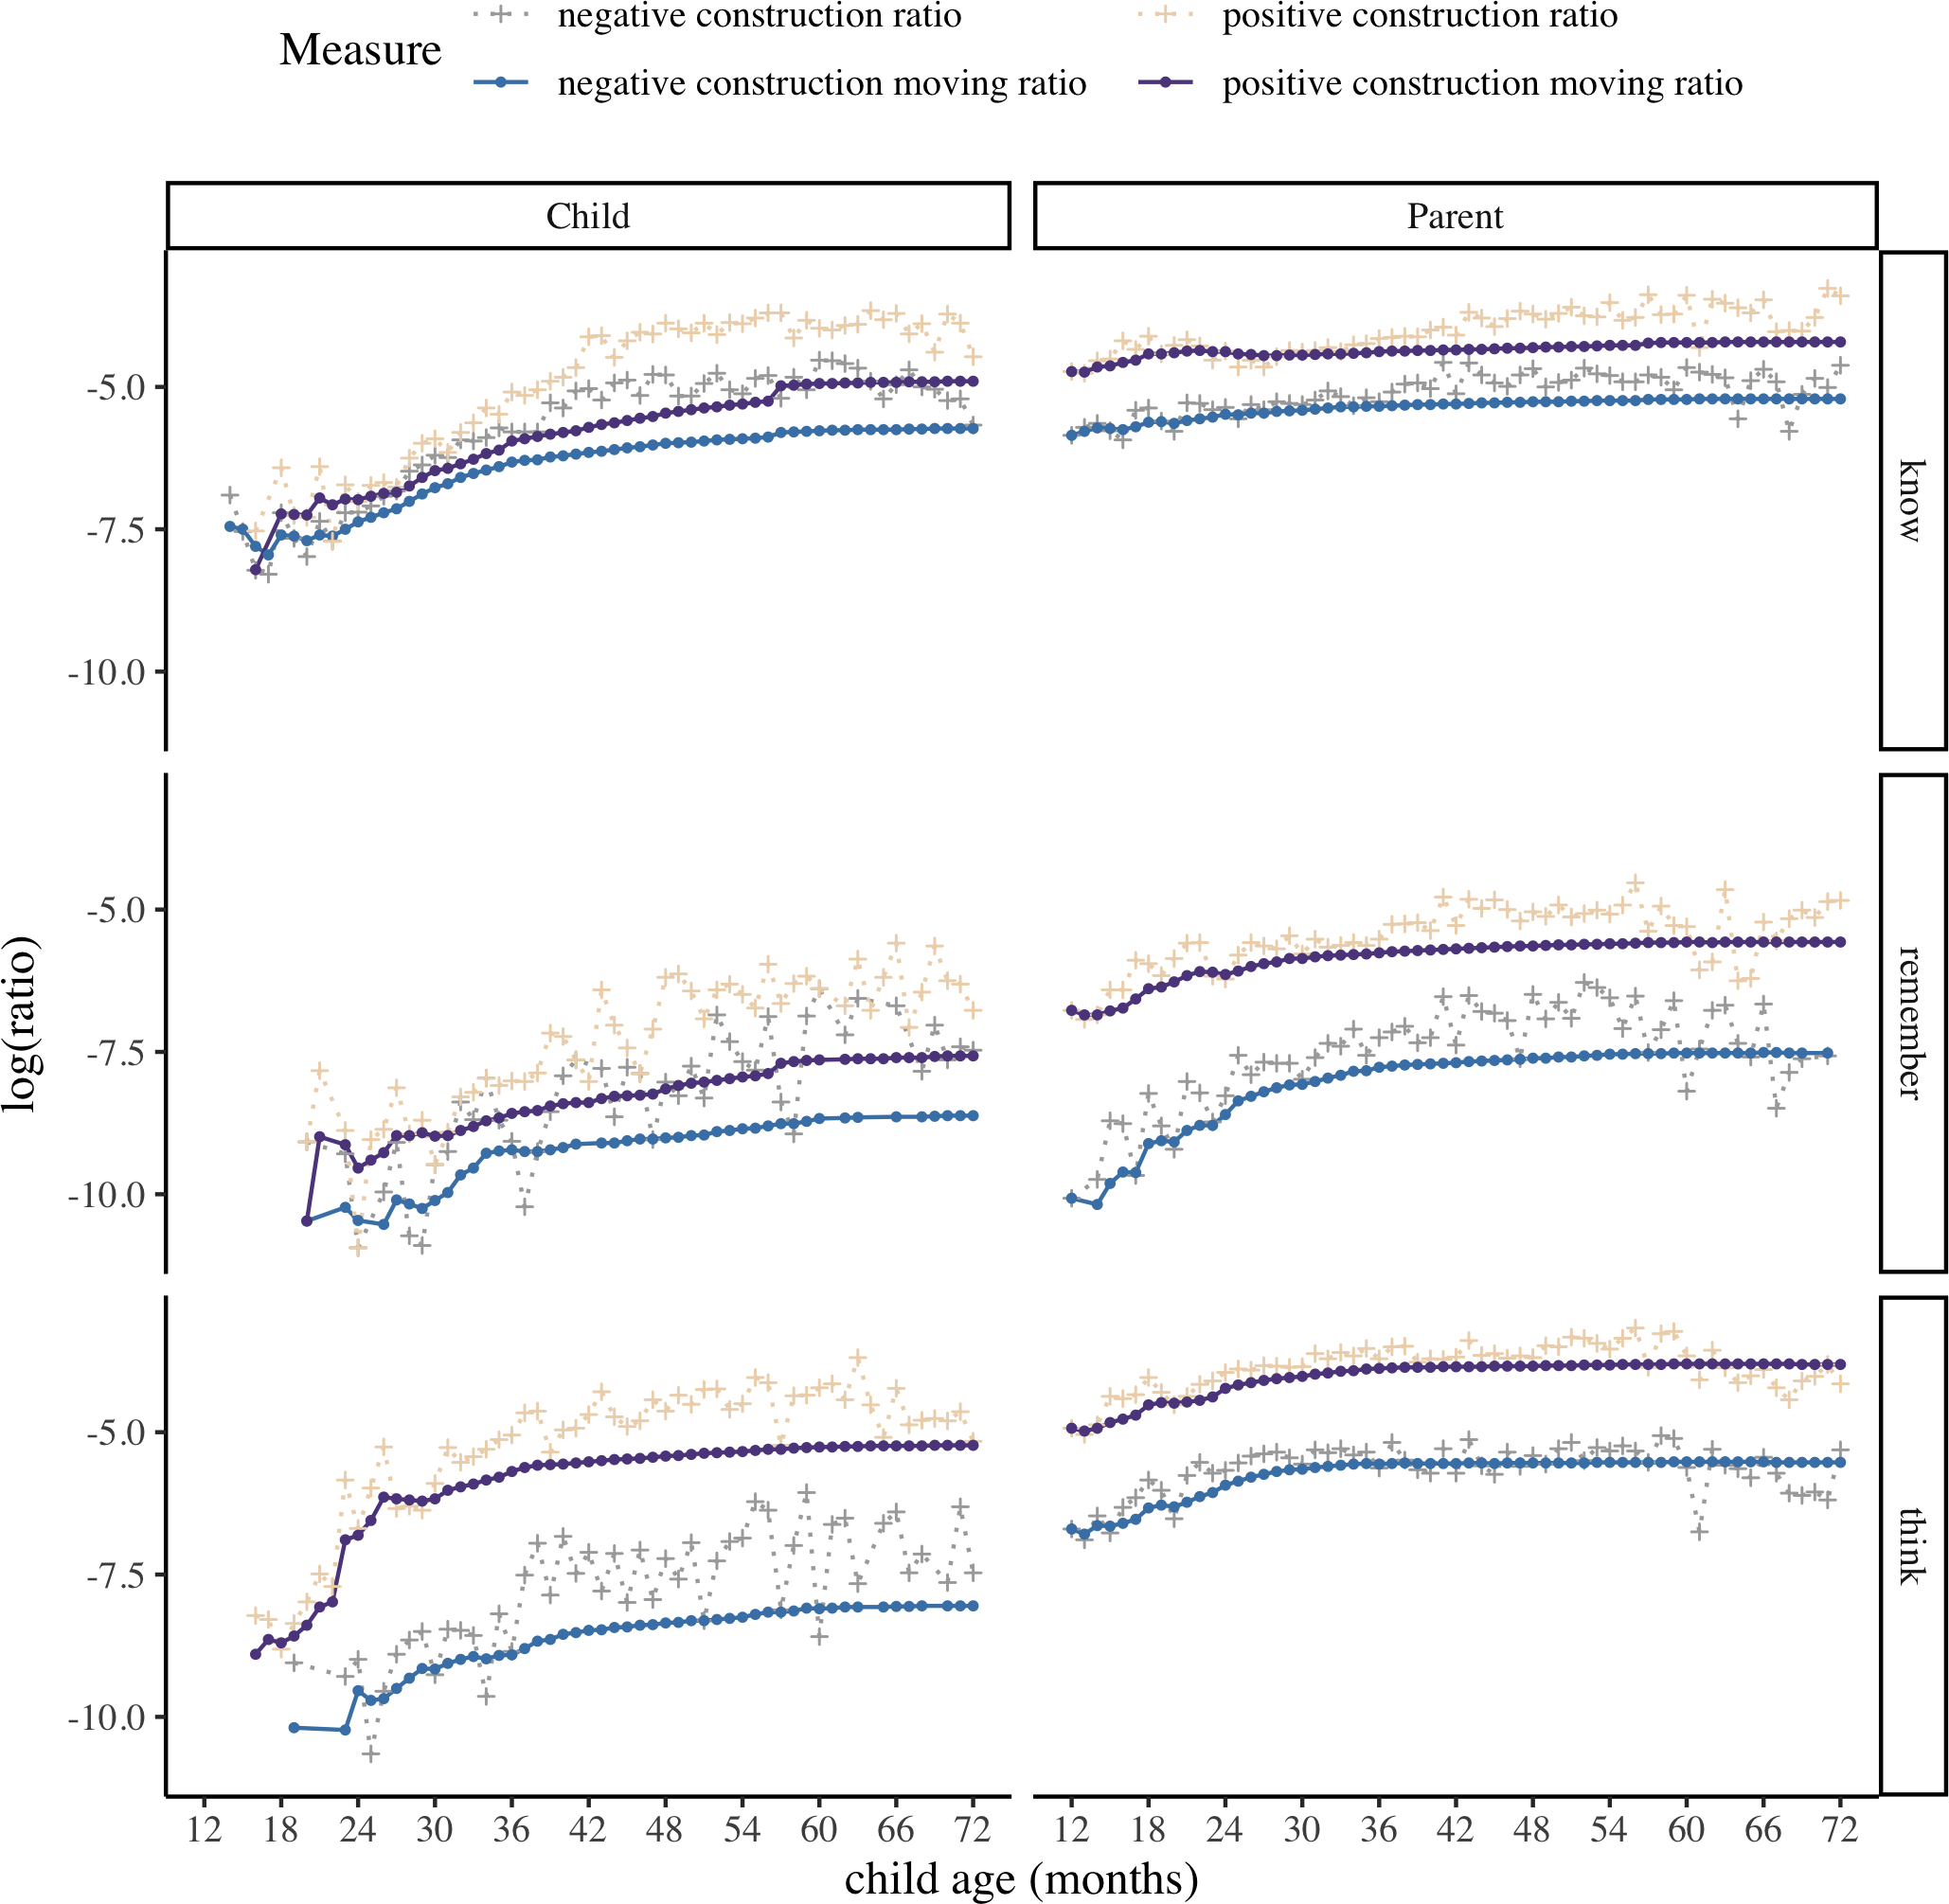
\includegraphics{neg_construction_article_files/figure-latex/epistemic-1} 

}

\caption{Cumulative production ratios for the production of epistemic negation at the sentence level for children between 12 to 72 months of age, and their parents. The y-axes are scaled differently for the panels to accommodate differences in production ratios.}\label{fig:epistemic}
\end{figure}

For epistemic negation at the discourse level, we examined interactions in which the antecedent utterances took any of the three head verbs: \emph{know}, \emph{remember} and \emph{think}, leading to a total of 547 utterances (child: 412; parent: 135). As shown in Figure \ref{fig:epistemicdiscourse}, children's production of \emph{no} to negate antecedent epistemic utterances increases rapidly between 18-36 months and is in general higher than the production ratio of parents'.

\begin{longtable}[]{@{}
  >{\raggedright\arraybackslash}p{(\columnwidth - 2\tabcolsep) * \real{0.4583}}
  >{\raggedright\arraybackslash}p{(\columnwidth - 2\tabcolsep) * \real{0.5417}}@{}}
\caption{\label{tab:epistem} Examples of discourse-level epistemic negation in children's and parents' speech.}\tabularnewline
\toprule\noalign{}
\begin{minipage}[b]{\linewidth}\raggedright
Epistemic (Negative)
\end{minipage} & \begin{minipage}[b]{\linewidth}\raggedright
Positive counterpart
\end{minipage} \\
\midrule\noalign{}
\endfirsthead
\toprule\noalign{}
\begin{minipage}[b]{\linewidth}\raggedright
Epistemic (Negative)
\end{minipage} & \begin{minipage}[b]{\linewidth}\raggedright
Positive counterpart
\end{minipage} \\
\midrule\noalign{}
\endhead
\bottomrule\noalign{}
\endlastfoot
Parent: \emph{do you know} & Child: \textbf{\emph{no}} \\
Parent: \emph{do you remember} & \textbf{\emph{no}} \emph{I do\textbf{n't}} \emph{remember it} \\
Child: \emph{does she think so} & Parent: \textbf{\emph{no}} \textbf{\emph{not}} \emph{really} \\
Child: \emph{do they know it's today} & \textbf{\emph{no}} \emph{I do\textbf{n't}} \emph{think so honey} \\
\end{longtable}

\begin{figure}[H]

{\centering 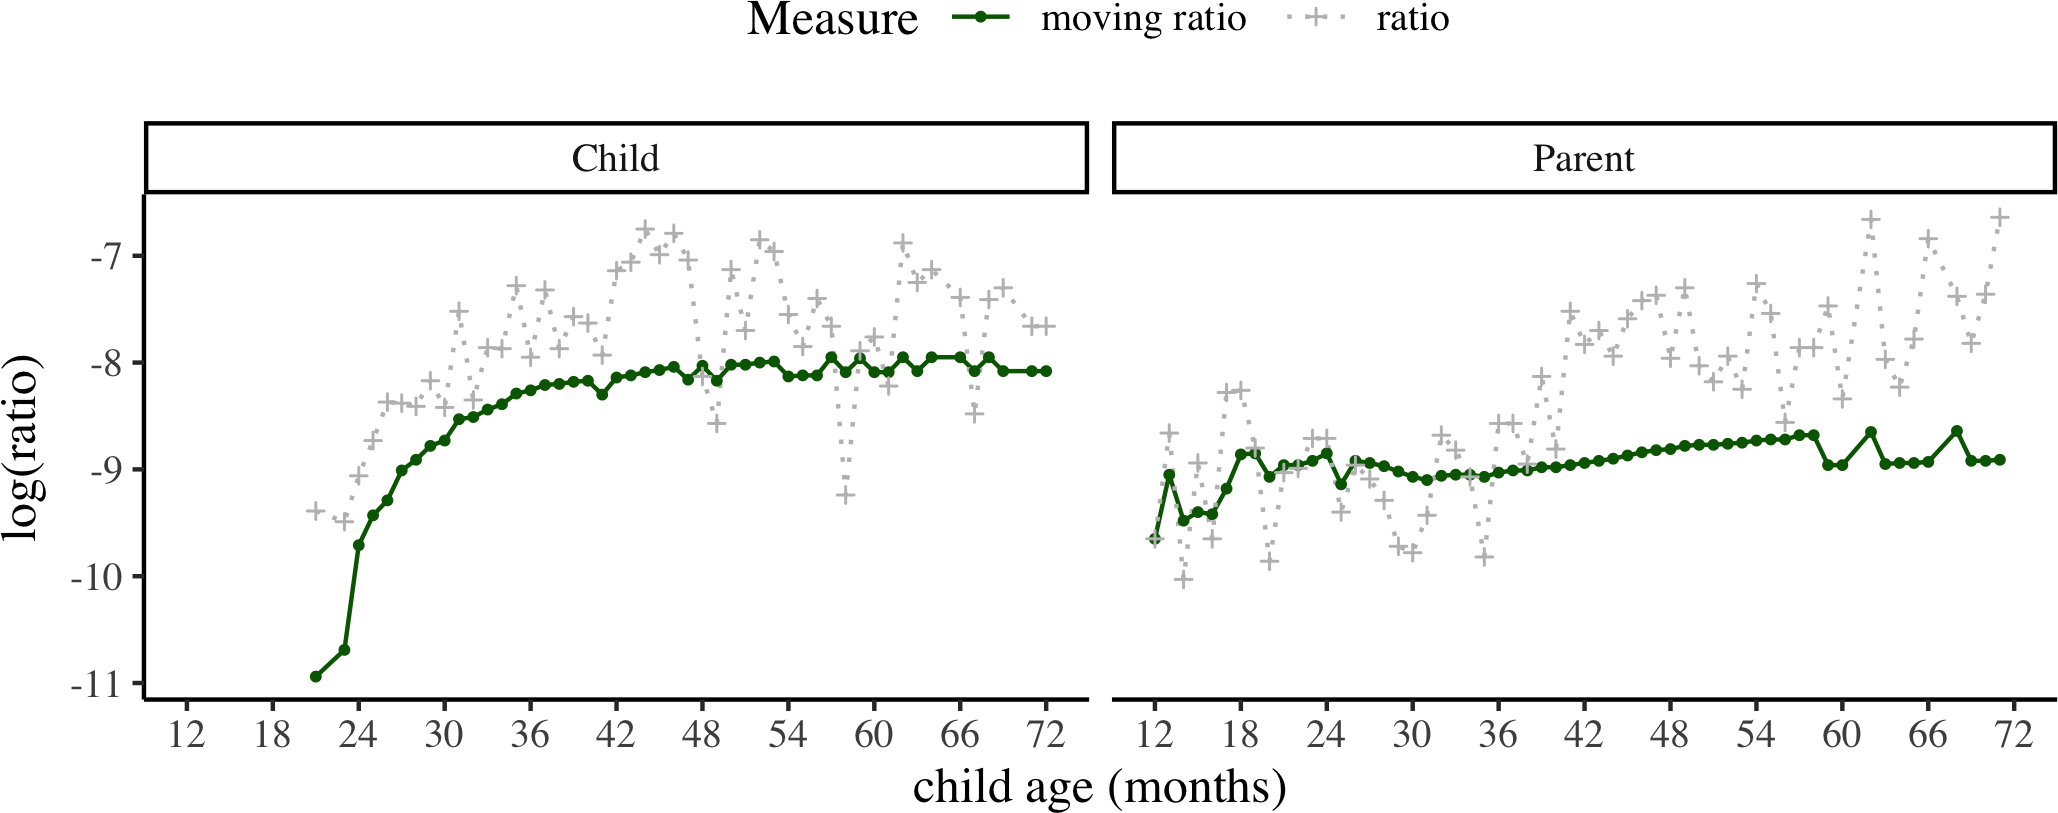
\includegraphics{neg_construction_article_files/figure-latex/epistemicdiscourse-1} 

}

\caption{Cumulative production ratios for the production of epistemic negation at the discourse level for children between 12 to 72 months of age, and their parents.}\label{fig:epistemicdiscourse}
\end{figure}

\subsubsection{Possession}\label{possession}

The last function we explored was possession. At the sentence level, for negative structures we selected cases where negative morphemes were combined with auxiliary verbs to modify head verbs with the lemma form \emph{have}, and the POS tag of these head verbs is all ``VERB''. We also included cases of which the syntactic head is a nominal predicate; the nominal predicate can either be a possessive pronoun (e.g., ``yours'') or a noun phrase with a possessive modifier (e.g., ``her book''). Table \ref{tab:possess} presents several examples. The number of negative utterances subjected to analysis for this function is 8,892 (child: 2,830; parent: 6,062). Again the positive counterparts share similar structures except without negation, leading to a total of 86,665 utterances (child: 27,730; parent: 58,935). One thing to note here is that for the positive structures with the head verb \emph{have}, we restricted our search to instances where the head verb takes a direct object (with the dependency relation \emph{obj}). This is to avoid potential parsing errors of utterances such as \emph{I have}, where the verb could be an auxiliary.

\begin{longtable}[]{@{}ll@{}}
\caption{\label{tab:possess} Examples of sentence-level possession (negative) and positive counterparts in children's speech.}\tabularnewline
\toprule\noalign{}
Posession (Negative) & Positive counterpart \\
\midrule\noalign{}
\endfirsthead
\toprule\noalign{}
Posession (Negative) & Positive counterpart \\
\midrule\noalign{}
\endhead
\bottomrule\noalign{}
\endlastfoot
\emph{I do\textbf{n't}} \emph{have it} & \emph{you have that} \\
\emph{you do\textbf{n't}} \emph{have my toy car} & \emph{she has it} \\
\textbf{\emph{not}} \emph{mine} & \emph{this is hers} \\
\textbf{\emph{not}} \emph{yours either} & \emph{mine mine mine} \\
\end{longtable}

Figure \ref{fig:possession} presents cumulative ratios of possession construction at the sentence level. Regardless of whether the utterances are negative or positive, the production trajectory in child speech appears to have notable differences depending on the syntactic head. When the instances are headed by \emph{have}, children increase their production between 18-36 months, a pattern that is present in both negative and positive constructions; yet children's production ratio consistently stays below parents' level across the developmental path. For utterances headed by possessive pronouns, on the other hand, children's production increases rapidly between 18-24 months and stays above parents' production level as early as 24 months of age.

\begin{figure}[H]

{\centering 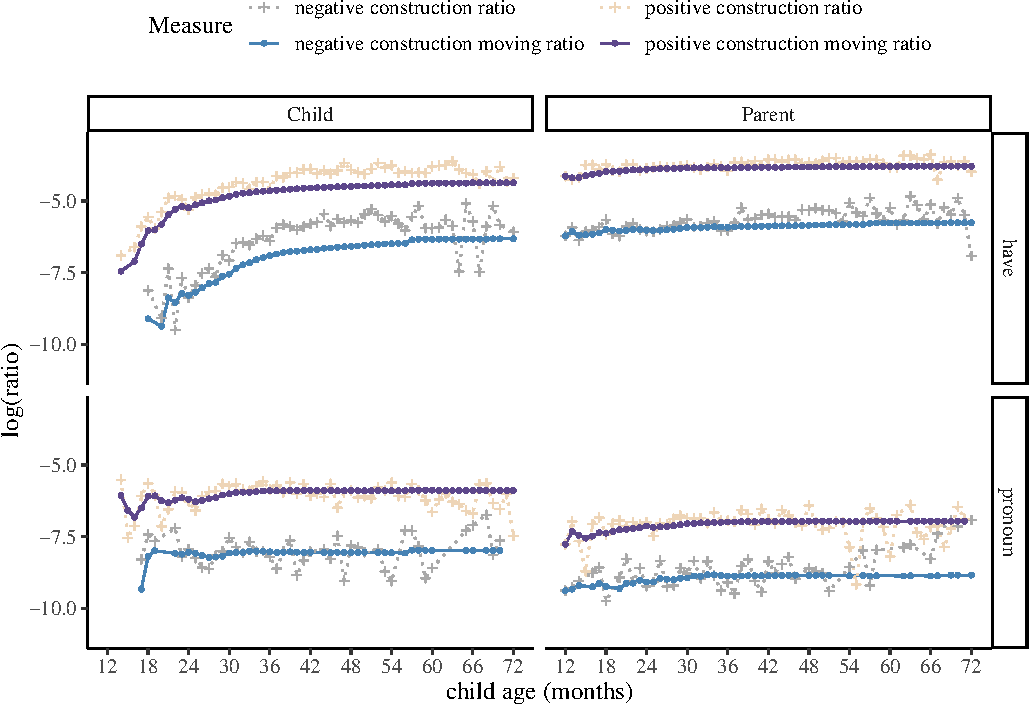
\includegraphics{neg_construction_article_files/figure-latex/possession-1} 

}

\caption{Cumulative production ratios for the production of possession at the sentence level for children between 12 to 72 months of age, and their parents. The y-axes are scaled differently for the panels to accommodate differences in production ratios.}\label{fig:possession}
\end{figure}

For discourse-level possessives, we selected antecedents of the negative response particle \emph{no} which themselves had structures similar to the negative and positive constructions of possession at the sentence level (Table \ref{tab:dispossess}). Based on Figure \ref{fig:possessiondiscourse}, the overall patterns indicate that children's production of possession at the discourse level increases gradually within the age range of 18 to 36 months; and their production ratio is mostly higher than that of parents.

\begin{longtable}[]{@{}
  >{\raggedright\arraybackslash}p{(\columnwidth - 2\tabcolsep) * \real{0.5526}}
  >{\raggedright\arraybackslash}p{(\columnwidth - 2\tabcolsep) * \real{0.4474}}@{}}
\caption{\label{tab:dispossess} Examples of discourse-level possession (negative) in children's and parents' speech.}\tabularnewline
\toprule\noalign{}
\begin{minipage}[b]{\linewidth}\raggedright
Antecedent
\end{minipage} & \begin{minipage}[b]{\linewidth}\raggedright
Utterance
\end{minipage} \\
\midrule\noalign{}
\endfirsthead
\toprule\noalign{}
\begin{minipage}[b]{\linewidth}\raggedright
Antecedent
\end{minipage} & \begin{minipage}[b]{\linewidth}\raggedright
Utterance
\end{minipage} \\
\midrule\noalign{}
\endhead
\bottomrule\noalign{}
\endlastfoot
Parent: \textbf{\emph{not}} \emph{yours} & Child: \textbf{\emph{no}} \emph{it's mine mine} \\
Parent: \emph{do you still have that picture} & Child: \textbf{\emph{no}} \\
Child: \textbf{\emph{not}} \emph{hers} & Parent: \textbf{\emph{no no}} \\
Child: \emph{mommy has it} & Parent: \textbf{\emph{no}} \emph{I do\textbf{n't}} \\
\end{longtable}

\begin{figure}[H]

{\centering 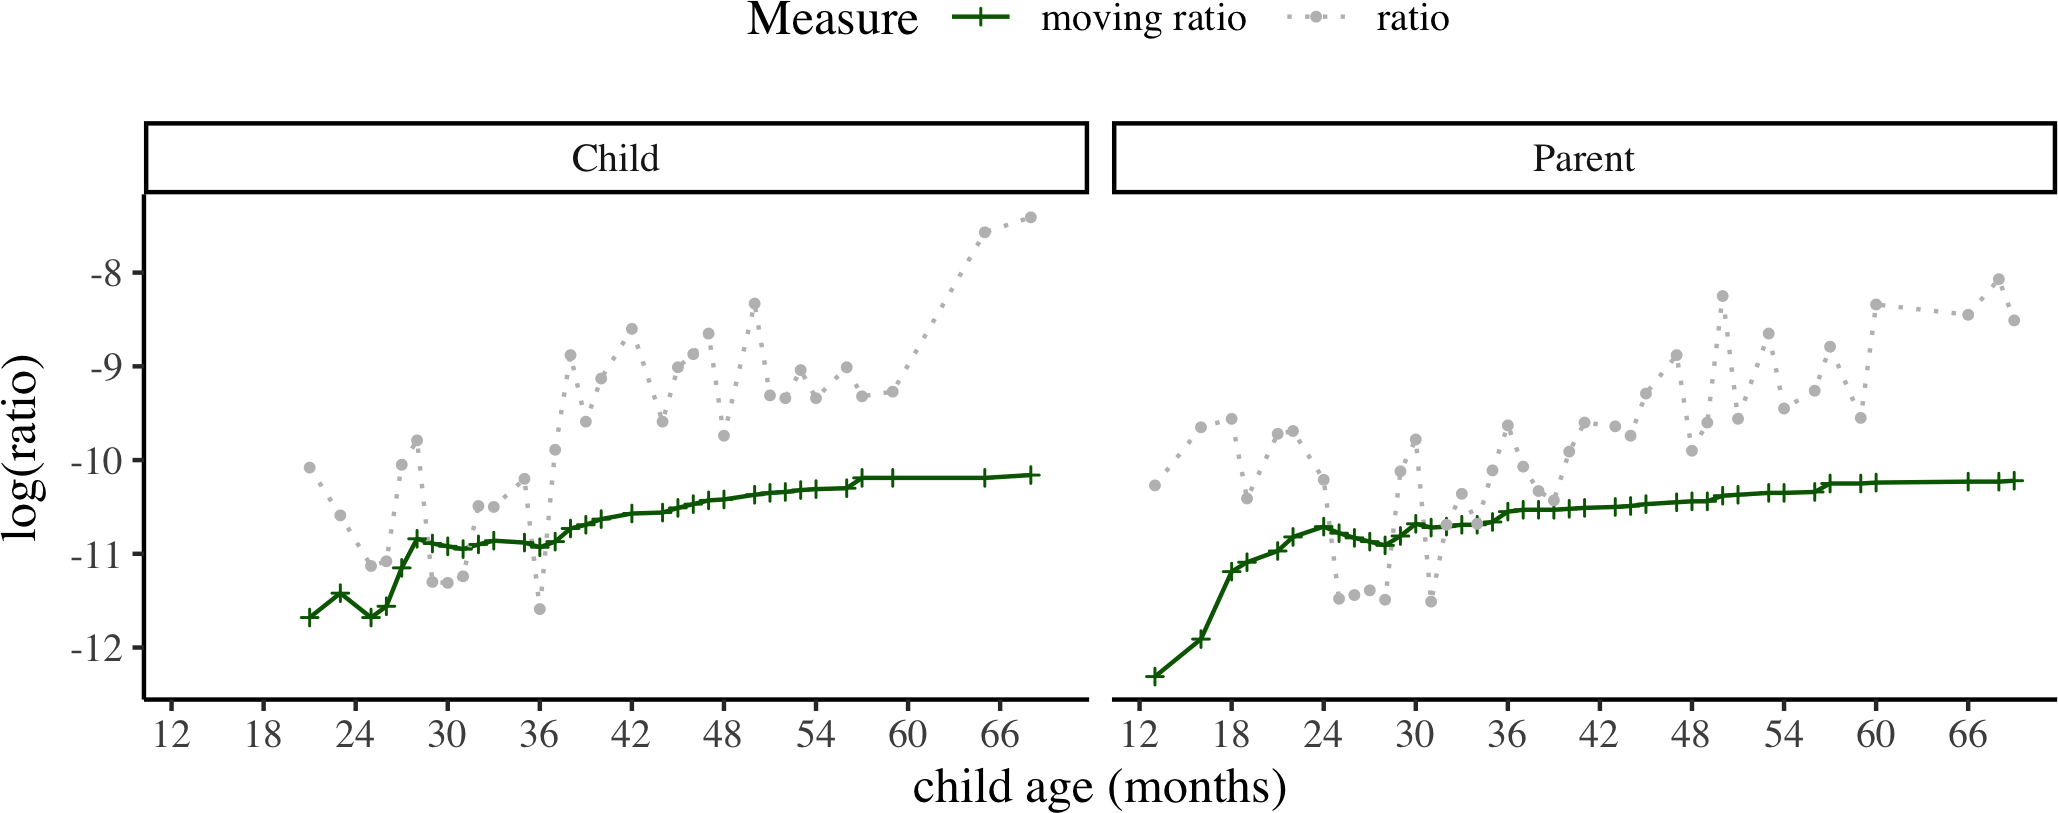
\includegraphics{neg_construction_article_files/figure-latex/possessiondiscourse-1} 

}

\caption{Cumulative production ratios for the production of possession at the discourse level for children between 12 to 72 months of age, and their parents.}\label{fig:possessiondiscourse}
\end{figure}

\subsubsection{All Constructions}\label{all-constructions}

In Figure \ref{fig:allneg}, we present the cumulative ratios of all our negative constructions at the sentence level for children (left panel) and parents (right panel). Parents produce most negative constructions at relatively constant rates across most of the age bins. Notable exceptions are labeling, epistemic, and prohibitions between 12-36 months. Parents increase their production of labeling and epistemic constructions in this period and their productions become more stable after 36 months. This obervation aligns with labeling and epistemic negation in child speech, which suggests that the production patterns in child speech for these two functions may be more influenced by interactions with parents, and vice versa as children grow to be more conversant and interactive. On the other hand, prohibition starts as one of the most frequent constructions at 12-18 months of age and ends up as the least frequently used construction after around 30 months. One reason for this trend may be that when children are younger, they need more guidance on their actions and parents provide such guidance with imperatives and commands, often in the form of prohibiting children from particular actions. As children grow older, verbal prohibitions become less necessary.

Most constructions begin to be produced by children in the 18-24 age range. Two functions, non-existence and prohibition, seem to emerge at later ages than others. With non-existence, even though there are examples between 18-24 months, the cumulative production ratios are fluctuating and discontinuous, instead of demonstrating a slow and steady increase as seen in most of the other functions. As described in previous sections, the data for non-existence before 25 months based on our corpus search is relatively sparse; it is possible that with larger corpora a clearer pattern may arise. With prohibition, we see a relatively smooth pattern. Children begin to produce them more regularly between 24-30 months and its rate of production stays below parents' levels. One explanation for this pattern is that parent-child interactions do not provide many contexts for children to prohibit parents. Overall by 36 months of age, children's production of most constructions starts to become stable.

\begin{figure}[H]

{\centering 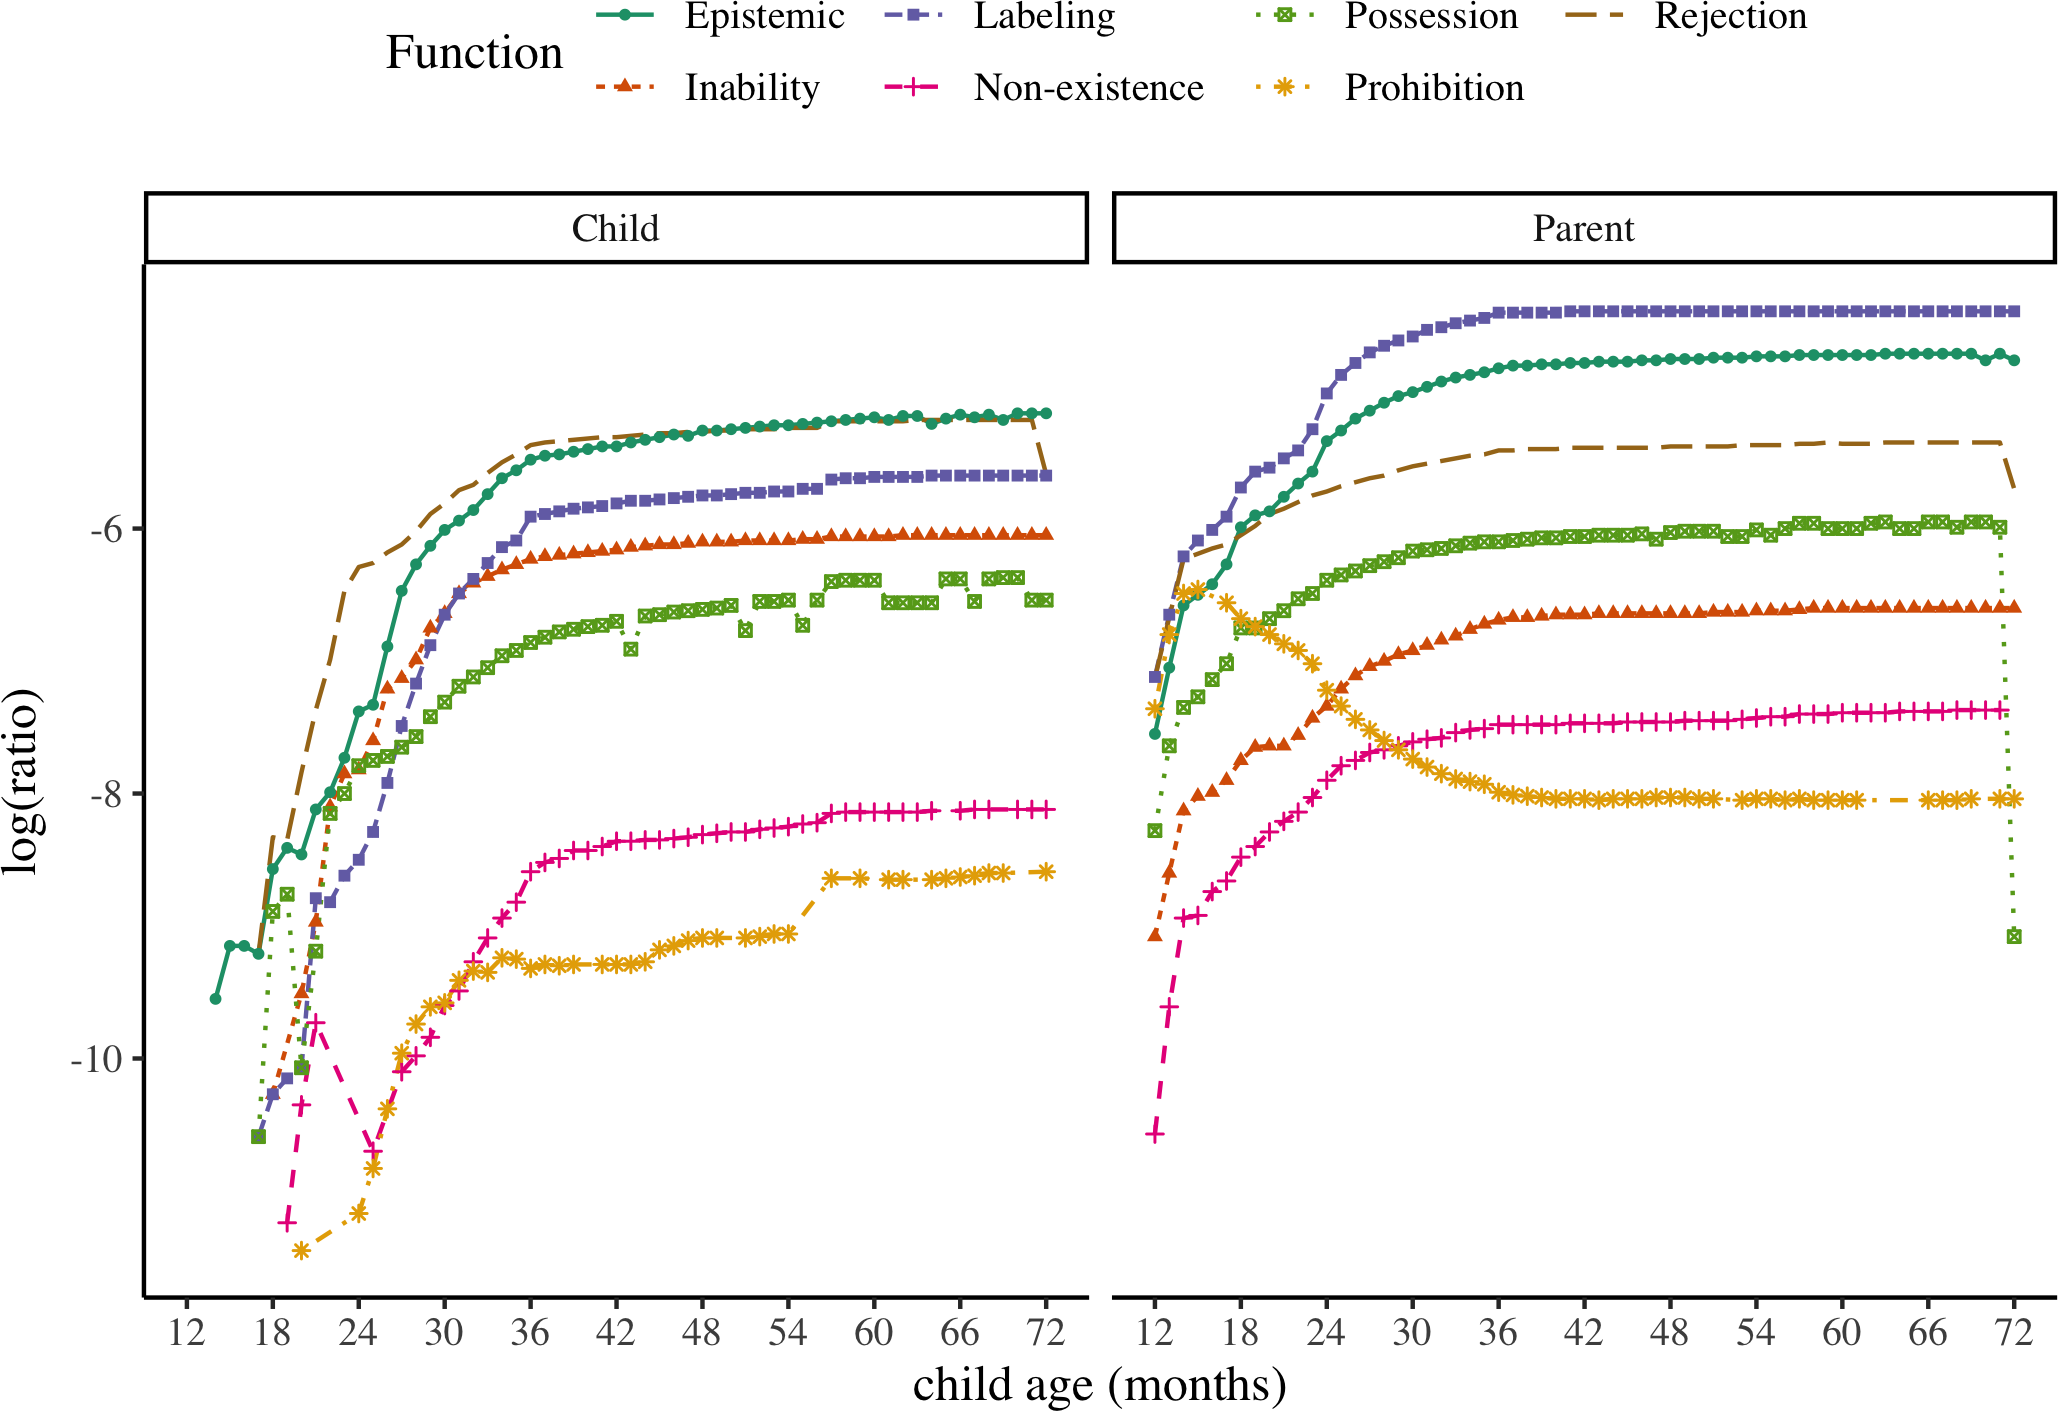
\includegraphics{neg_construction_article_files/figure-latex/allneg-1} 

}

\caption{Cumulative production ratios for all negative responses at the sentence level.}\label{fig:allneg}
\end{figure}

\begin{figure}[H]

{\centering \includegraphics{neg_construction_article_files/figure-latex/allnegagerestricted-1} 

}

\caption{Cumulative production ratios for all negative constructions at the sentence level when children are between 12-24 months of age.}\label{fig:allnegagerestricted}
\end{figure}

Figure \ref{fig:allpos} shows the cumulative ratios of all positive counterparts to our negative constructions at the sentence level for children (left panel) and parents (right panel). The production of the positive instances in parent speech for almost all constructions is stable. Notable exceptions are labeling and positive counterparts to prohibitions (positive imperatives) between 12-30 months. Similar to negative instances of labeling, positive instances increase in frequency between 12-30 months but remain constant after. Positive imperatives are produced much more frequently between 12-36 months, but their production decreases later. This pattern mirrors what we see in Figure \ref{fig:allneg} with (negative) prohibitions, that the usage of imperatives in interactions potentially becomes less necessary as children grow older.

All positive counterparts to our negative constructions being to be produced by children between the age range of 12-18 months. By 36 months, almost all positive constructions are being produced at a relatively constant rate close to parents' levels. Another noteworthy pattern is the relative high frequency of positive counterparts to prohibitions in the 12-24 months age period. In contrast to the production of (negative) prohibitions, positive imperatives are produced with high frequency even before 24 months of age. In other words, even though children do not frequently prohibit parents, they seem to be frequently ordering or commanding parents to do things for them; a finding that would not surprise many parents and caregivers!

\begin{figure}[H]

{\centering 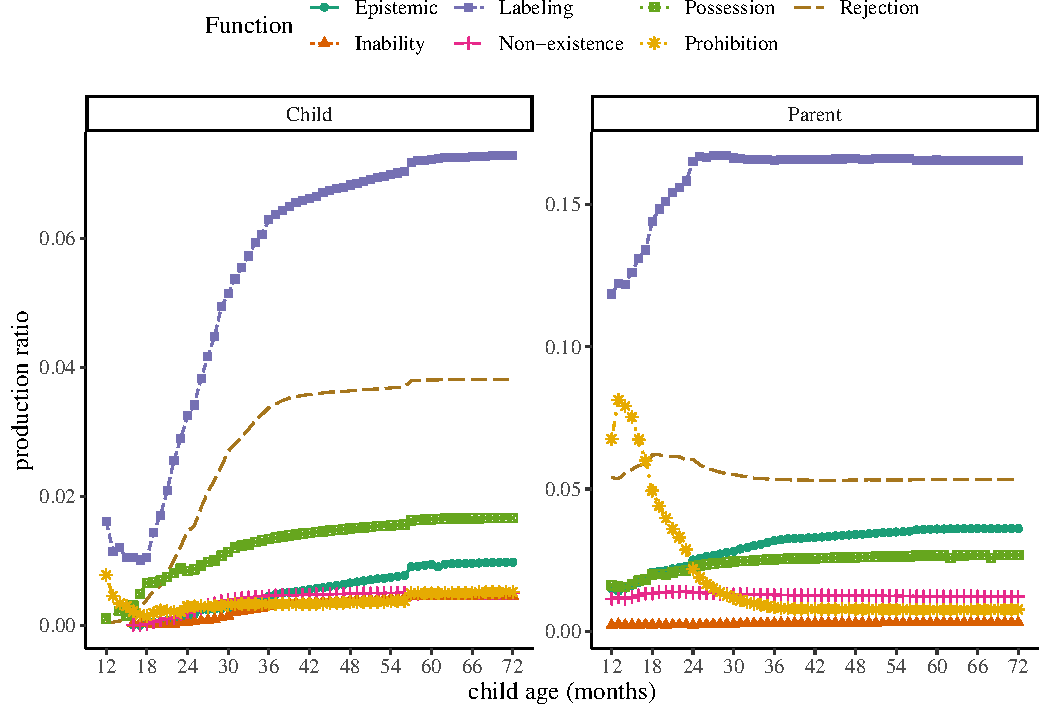
\includegraphics{neg_construction_article_files/figure-latex/allpos-1} 

}

\caption{Cumulative production ratios for the positive counterparts to all negative constructions at the sentence level.}\label{fig:allpos}
\end{figure}

\begin{figure}[H]

{\centering \includegraphics{neg_construction_article_files/figure-latex/allposagerestricted-1} 

}

\caption{Cumulative productive ratios for the positive counpterparts to all negative constructions at the sentence level when children are between 12-24 months of age.}\label{fig:allposagerestricted}
\end{figure}

Summarizing children's production patterns at the sentence level, we find earliest instances of children producing the negative constructions in our study in the 18-14 months age range. The positive counterparts to our negative constructions begin to be produced slightly earlier and in the 12-18 age range. For both negative constructions and their positive counterparts, children's ratio of production increases substantially from 18 to 36 months, then starts to become stable (increase very slowly) after 36 months of age.

Finally, Figure \ref{fig:alldiscourse} illustrates the cumulative ratios of all negative responses at the discourse level. Observations for parents' speech on the right again demonstrates a relatively constant rate of production after 36 months. Before 36 months, however, most constructions show a gradual increase with the exception of prohibition. Parents start with more frequent ``no!''-responses to imperatives produced by children, but the frequency of these negative responses drops to a relatively low and stable level after children are 36 months of age; this pattern again corresponds to parents' production of subjectless imperatives in Figure \ref{fig:allneg} and Figure \ref{fig:allpos}.

\begin{figure}[H]

{\centering 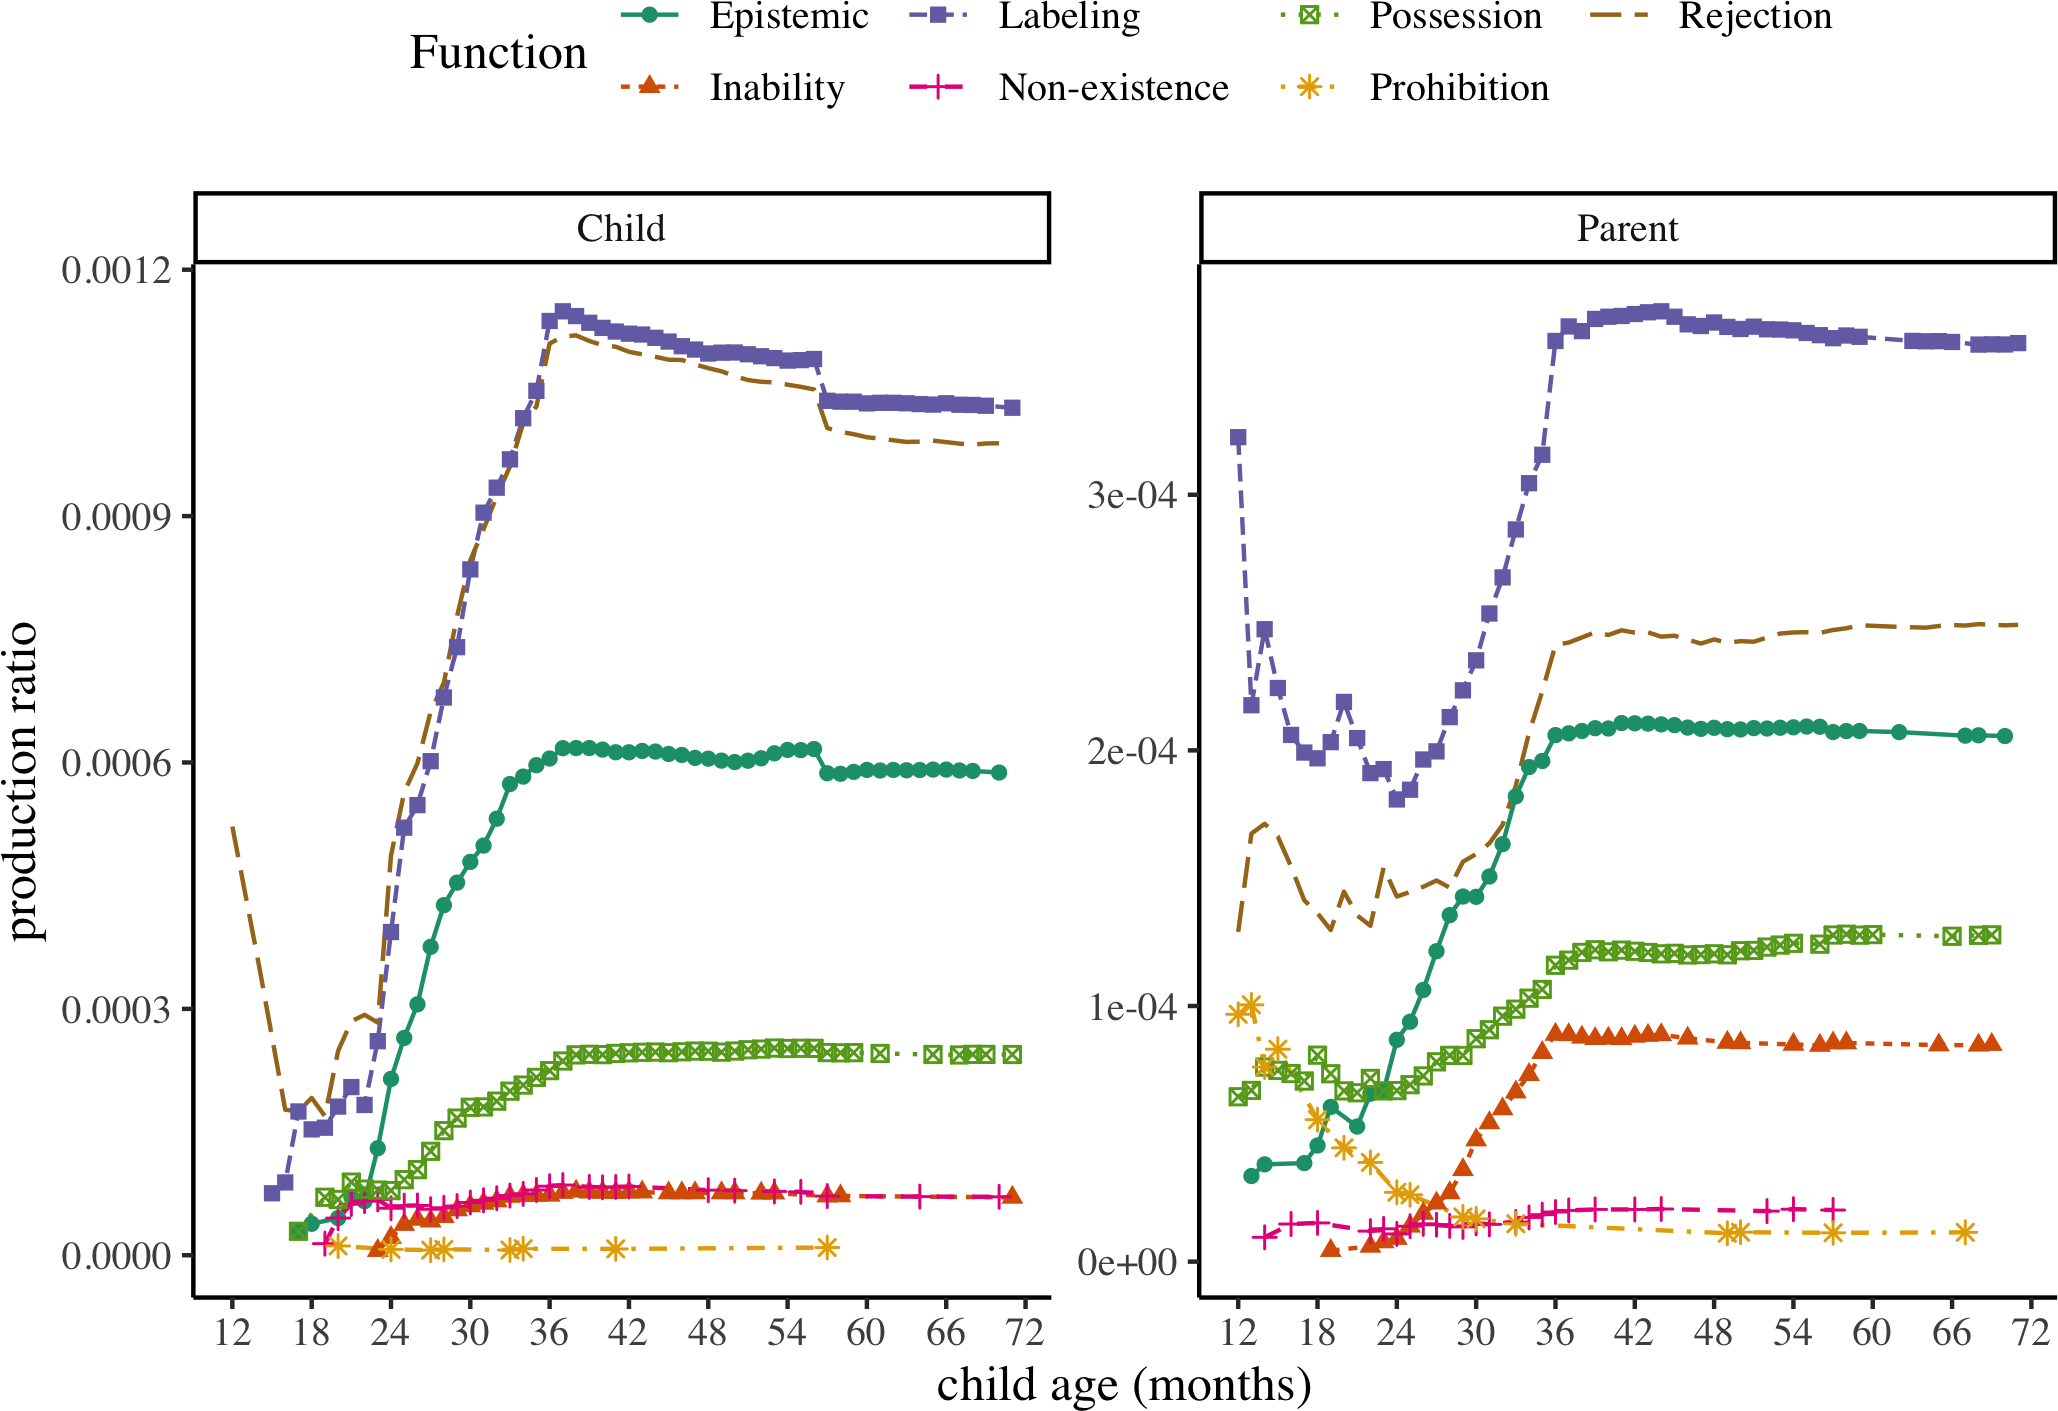
\includegraphics{neg_construction_article_files/figure-latex/alldiscourse-1} 

}

\caption{Cumulative production ratios for all negative constructions at the discourse level.}\label{fig:alldiscourse}
\end{figure}

\subsection{Statistical Modeling}\label{statistical-modeling}

In order to model the overall production trajectories of different negative constructions, we adopted developmental growth curve analysis (Kemper, Rice, \& Chen, 1995; Van Veen, Evers-Vermeul, Sanders, \& Van den Bergh, 2009). In particular, we used Gompertz curves (Boedeker, 2021; Gompertz, 1825; Panik, 2014) to model the cumulative ratio \(R_{c,t}\) for a construction \(c\) at a monthly age bin \(t\) using three parameters: the upper asymptote \(a\), the maximum growth rate \(r\), and the inflection point \(i\) along the x-axis (\(e\) is Euler's number):

\(R_{c, t} = a \times e^{-e^{(-r \times (t - i))}}\)

We chose Gompertz curves because they best satisfy our assumptions and observations regarding children's production of negative constructions. First, using cumulative ratios as the main measure guarantees an upper threshold or limit that the measure could reach (i.e.~total proportion of a construction produced) by the end of the developmental period. Second, children start with no negative utterances and slowly increase their production. Third, this increase in production can be nonlinear. Similarly, Gompertz curves have an upper asymptote \(a\) and in the standard form start from zero. They also assume a possibly non-linear growth. The ratio increases rapidly at first until it reaches peak growth of \(r\) at time interval \(i\), then the growth slows down until the ratio reaches the stable maximum threshold estimated by the upper asymptote \(a\). The rapid growth period and the slowdown period before and after the inflection point \(i\) can be asymmetrical.

There are three main points along a growth curve that can be informative regarding the forward and backward shift of the curve along the x-axis (i.e.~age): first, the beginning of growth, often called the ``lag time'' or \(\lambda\) under a different parameterization of the formula above; second, the inflection point \(i\) discussed above where maximum growth is reached; and third, the point along the x-axis at which the curve reaches its asymptote \(a\). For language production, the first measure provides an estimate of when a particular word or construction is first produced by some children in a corpus. It is suitable for assessing earliest production but it may be biased by children who start early. The second measure provides an estimate of when the construction has reached maximum increase in its ratio. It is likely a more robust and conservative measure of children's production of a word or a construction but it will likely underestimate earliest instances of production (as opposed to the first measure, i.e.~lag time). Finally, the third measure estimates the age at which the ratio of producing a construction reaches a stable level and does not change anymore. This measure may be more suitable as a measure of stability in production for a particular word or construction. In this study, we use the inflection point \(i\) as our main measure of forward/backward shift for growth curves to first, address the data sparsity issue in early production which makes estimating lag time much more difficult, and second, provide a more conservative estimate of children's production overall and avoid a bias for early starters.

We used the statistical package \(brms\) to implement our Gompertz growth curve analysis. We fit separate growth curves to each negative and positive construction at the sentence and discourse levels. We used uniform priors with appropriate bounds for the three parameters of our Gompertz models. For the asymptote we kept the values between 0 and 10 because we did not observe relative frequencies above 7 (per thousand) for any construction. For the growth rates we kept the values between 0 and 3 given that growth rate will always be positive and that values above 3 represent very rapid and sharp developments unlike what we have observed. All estimated growth rates were below 1. And finally for the point of inflection we kept the values between 12 and 72 given that this is children's age range in this study. Since we did not have enough data to capture the developmental paths of individual children, the logistic curves did not have random effects and were fit at the population level for each communicative function. Each model ran 4 chains with 4000 iterations each and 2000 of them as warm-up. 95\% credible intervals for each parameter were derived from their respective posterior distribution.

\(a\) \(\sim\) \(Uniform(0, 10)\)

\(r\) \(\sim\) \(Uniform(0, 3)\)

\(i\) \(\sim\) \(Uniform(12, 72)\)

\begin{figure}[H]

{\centering \includegraphics{neg_construction_article_files/figure-latex/sentencePredictionPlot-1} 

}

\caption{Predicted Gompertz growth curves for sentence-level negative constructions. The x-axis is age in months, and the y-axis represents cumulative production ratio per thousand utterances.}\label{fig:sentencePredictionPlot}
\end{figure}

First we look at the predictions of our models for sentence-level negation, which reflect children's productive capacities. Figure \ref{fig:sentencePredictionPlot} presents the predicted growth curves for the seven sentence-level negative constructions in children's speech. While the curves differ substantially in their asymptote (the upper threshold for the production), they seem to have similar onset of production around 20 months of age or slightly earlier. Figure \ref{fig:valencePredictionPlot} compares the positive (green) and negative (red) growth curves for the same constructions. The negative curves always have lower asymptotes compared to the positive curves, which means positive constructions constitute larger proportions of children's speech compared to their negative counterparts. More importantly, the onsets for the negative curves are always at or after the positive curves. This suggests that on average, negative constructions are produced after or at around the same age as their positive counterparts.

\begin{figure}[H]

{\centering \includegraphics{neg_construction_article_files/figure-latex/valencePredictionPlot-1} 

}

\caption{Predicted Gompertz growth curves for sentence-level positive (green) vs. negative (red) constructions. The x-axis is age in months, and the y-axis represents cumulative production ratio per thousand utterances.}\label{fig:valencePredictionPlot}
\end{figure}

Figure \ref{fig:negativePositiveInflectionPlot} shows model estimates for the inflection points for sentence-level positive and negative growth curves. The inflection point is the age at which children's production ratio for a construction has reached maximum growth and starts to slow down. The inflection point also represents the forward shift of the curves. The inflection points for most positive constructions are earlier than their negative counterpart. The two exceptions are epistemic and inability constructions, which have very frequent negative usages early on. The inflection points for most negative constructions fall between 26 and 32 months of age. This is the age range where several experimental studies report successful comprehension of negation in a wide range of tasks using different constructions such as labeling (e.g.~it's not a dog) or negative predicative PPs (e.g.~it's not in the bucket) (K. Austin, Theakston, Lieven, \& Tomasello, 2014; De Villiers \& Flusberg, 1975; Feiman, Mody, Sanborn, \& Carey, 2017; Hummer, Wimmer, \& Antes, 1993; Reuter, Feiman, \& Snedeker, 2018). It is also the age range for many production studies that report the presence of different communicative functions discussed in our literature review earlier.

\begin{figure}[H]

{\centering \includegraphics{neg_construction_article_files/figure-latex/negativePositiveInflectionPlot-1} 

}

\caption{Estimates with 95 percent credible intervals for inflection points of the Gompertz growth curves for sentence-level positive (green) and negative constructions. The x-axis is age in months, and the y-axis represents seven negative constructions.}\label{fig:negativePositiveInflectionPlot}
\end{figure}

Next we consider the predictions of our models for discourse-level negation. Figure \ref{fig:discoursePredictionPlot} shows the predicted growth curves for children's discourse level negation. Similar to sentence-level growth curves, we see different asymptotes for each construction, suggesting that different constructions are used and negated at different proportions. However, similar to what we saw with sentence-level negation, these constructions seem to start recieving discourse level negative responses around 20 months of age and in some cases slightly earlier. The curve for the rejection construction leaves this possibility open that rejections are negated at the discourse level much earlier than the other constructions. However, we need much more data in the early age range of 12-30 months to be able to assess this hypothesis with more confidence.

\begin{figure}[H]

{\centering \includegraphics{neg_construction_article_files/figure-latex/discoursePredictionPlot-1} 

}

\caption{Predicted Gompertz growth curves for discourse-level negative constructions. The x-axis is age in months, and the y-axis represents cumulative production ratio per thousand utterances.}\label{fig:discoursePredictionPlot}
\end{figure}

Figure \ref{fig:sentenceDiscoursePredictionPlot} compares the growth curves for discourse-level negative responses to each construction with the growth curves for the sentence-level production of that construction. Across all constructions, their discourse-level curves show lower asymptotes than sentence-level curves. At the discourse-level, almost all constructions show similar onset of production around 20-months or slightly earlier. For episetmic and inability constructions, the sentence level productions seem to appear slightly earlier than discourse level productions. For rejections, on the other hand, discourse-level prodution of negation seems to start slightly earlier. However, for more accurate estimates we need denser corpora in the 12-30 months age range.

\begin{figure}[H]

{\centering \includegraphics{neg_construction_article_files/figure-latex/sentenceDiscoursePredictionPlot-1} 

}

\caption{Predicted Gompertz growth curves for children's sentence-level (green) vs discourse-level (red) negation. The x-axis is age in months, and the y-axis represents cumulative production ratio per thousand utterances.}\label{fig:sentenceDiscoursePredictionPlot}
\end{figure}

Finally, Figure \ref{fig:sentenceDiscourseInflectionPlot} shows the model estimates for the inflection points of the discourse-level (red) and sentence-level (green) negative growth curves. Overall, discourse-level curves reach their maximum growth earlier than sentence-level curves. For most discourse-level curves, the inflection point is around 24 months of age. Prohibition and non-existence constructions show more uncertain estimates likely due to the limited amount of data available across age bins.

\begin{figure}[H]

{\centering \includegraphics{neg_construction_article_files/figure-latex/sentenceDiscourseInflectionPlot-1} 

}

\caption{Estimates with 95 percent credible intervals for inflection points of the Gompertz growth curves for discourse-level (red) and sentence-level (green) negative constructions. The x-axis is age in months, and the y-axis represents seven negative constructions.}\label{fig:sentenceDiscourseInflectionPlot}
\end{figure}

\section{Conclusion}\label{conclusion}

In this study, we used the largest available collection of English child language corpora to examine the production trajectories of seven negative constructions that tend to convey seven negative communicative functions previously discussed in the literature on the development of negation. We used growth curves to model the emergence and development of these constructions in children's linguistic productions between one and six years of age. As a proxy for their comprehension, we also conducted the same analyses with parents' constructions that children responded to with discourse level negation (\emph{no}). Overall, we did not find strong evidence for large-scale population-level stages in children's development of negative communicative functions. Both sentence-level and discourse-level negation as proxies for production and comprehension of negation found that almost all negative constructions have their onset around the 18-22 months window. The point of maximum growth for discourse level negation was estimated at around 24 months and for sentence level negation between 26-32 months. The comparison of negative and positive curves showed the production of negative constructions emerges at or after their positive counterpart.

Before discussing the implications of our study, we would like to emphasize its limitations. First, prior studies have used small-scale human annotation that in addition to the utterance construction, takes contextual information into account. These studies also considered two-word or three-word utterances such as \emph{no noise} and \emph{no more milk} which are more ambiguous with respect to their communicative function. Our study, on the other hand, did not use such two-word or three-word utterances and instead used specific constructions that convey negative communicative functions less ambiguously. Since the population-level stage-hypothesis should apply to all types of negative utterances, we chose to test it at a larger scale with automatic annotation of these less ambiguous constructions. While, our findings are compatible with small-scale human annotation studies of de Villiers and de Villiers (1979) and Nordmeyer and Frank (2018), they need to be corroborated with large scale human annotation of negative utterances to make sure the results do not depend on our methodological choices.

Second, the methods used in this paper are best suited for detecting large-scale population-level developmental patterns in children's productions. Due to data sparsity, our study cannot determine small-scale stages that are separated only by a few days or weeks. We cannot corroborate or refute such quick developmental stages using available corpus data and methods. Future research can use dense data collection in the age ranges of 18-22 or 18-30 months from a large number of children to investigate small-scale developmental stages. Since we do not have individual-level developmental data, our study cannot detect individual-level stages either. As we have emphasized throughout the paper, our methods are suitable for detecting large-scale population-level stages, which were the focus of prior research as well. Finally, the methods used in this paper are best suited for directly assessing children's productions. Our estimates of children's comprehension by analyzing their discourse-level negative responses to parents' utterances are only indirect measures. Therefore, any conclusion regarding children's comprehension must be treated with caution. For detecting developmental stages in children's comprehension, we consider experimental studies focused on particular age ranges to be most suitable. Only in combination with such experimental studies can the results on children's comprehension in this study be appropriately interpreted.

Third, we did not study communicative functions of negation exhaustively. Nor did we discuss all constructions that can be used to convey the communicative functions in our study. Given a communicative function, there are many constructions that can potentially convey it more literally (semantically) or figuratively (pragmatically). For example, both \emph{I cannot do \ldots{}} and \emph{this is difficult} can convey inability. However, the first construction does this more literally and more reliably. In this study, we have specifically focused on constructions that more reliably convey certain negative communicative functions hypothesized to develop in stages. If negative communicative functions develop in population-level stages (conceptually, as well as in comprehension and production as prior literature suggested), then we expect to see stages in the sample of constructions that typically convey such communicative functions as well. While our study addresses this particular hypothesis and the particular constructions that we studied, the results and conclusions cannot be generalized to the development of all negative communicative functions or all constructions that convey them. They also leave several other nativist and empiricist hypotheses as open possibilities that we discuss next.

What are the implications of these results for the logical empiricist and nativist approaches? Remember that we discussed several empiricist and nativist accounts of negation development depending on whether they predicted stages in comprehension or production (Figure \ref{fig:theory}). The results in this study are most compatible with the absence of population-level developmental stages for negative communicative functions in children's production, and possibly comprehension, although as we pointed out earlier the implications for comprehension should be treated with caution and interpreted only in tandem with focused experimental studies. Going back to \ref{fig:theory}, the empiricist (1A) and nativist (1B) accounts most compatible with this conclusion are those that do not predict population-level stages in production (3B) and possibly comprehension (2B). Under these two accounts, children may vary in the order that they comprehend or produce different negative construction or communicative functions. Under the nativist account, they need to solve a mapping problem and find out which morphemes correspond to their innate concept of abstract negation. In the empiricist account, children will induce abstract negation from the communicative functions they comprehend and produce regardless of the order of exposure or acquisition.

Determining whether the comprehension of negative communicative functions develops in population-level stages or not requires experimental research. It is possible that children comprehend communicative functions in fixed stages, yet these stages are not reflected in production data that can be captured by our corpus methods. They may require experiments designed for testing the comprehension of different negative communicative functions in the 18-30 months age range. We strongly encourage researchers to pursue such experimental studies. The discovery of population-level developmental stages in comprehension would rule out the two nativist and empiricist accounts discussed above, and allow for two different ones: 1. an empiricist account (1A), in which abstract negation is induced in ordered stages from concrete communicative functions (2A), but children's production does not reflect this due to a production bottleneck (3B). In other words, by the time children start their production of negation, the comprehension of communicative functions and inducing abstract negation is already complete; and 2. a nativist account (1B), in which the ordered stages in comprehension are the result of an information bottleneck (2A) (Gomes et al., 2023; McDermott-Hinman \& Feiman, In Press). Children's production, however, would show no signs of these stages due to a production bottleneck (3B).

Finally, it is possible that population-level small-scale and quick stages in production exist but have not been detected by the methods used in this study. Detecting population-level small-scale and quick stages requires very dense data collection from a large number of children in the 18-22 or 12-30 months age range. This type of data is currently not available but future research can provide such a dataset that would be generally valuable to research on children's early language acquisition. Whether in comprehension and production, our study highlights the importance of focused data collection in the 18-30 age range for future research on the development of negation.

The emergence of negation around 18-22 months is consistent with prior experimental and observational studies. Carvalho, Crimon, Barrault, Trueswell, and Christophe (2021) tested 18- and 24-month-old children in an experimental paradigm that tested the role of negation in early word learning. They presented novel labels for novel objects and actions to 18-month-old children, then tested their looking times on negative sentences that were either true or false given the presented visual stimuli. They also presented novel labels for objects to 24-month-olds using positive or negative statements (e.g.~``It's a bamoule!'' vs.~``It's not a bamoule!''). They found that both groups were capable of using negation to understand the intended objects in such labeling constructions. Some other studies have also confirmed children's successful comprehension of negation around 27 months or slightly older (K. Austin et al., 2014; De Villiers \& Flusberg, 1975; Feiman et al., 2017; Hummer et al., 1993; Reuter et al., 2018). In this study, and using different methods than prior literature, namely automatic detection and classification of negative constructions in children's speech and growth curve modeling, we provided further evidence that the 18-22 months window is where we expect early comprehension and production of negation to emerge. We believe that future research in this age range can help us tease apart the theoretical possibilities discussed above and converge on a unified account for the development of negation in child language.

\phantomsection\label{refs}
\begin{CSLReferences}{1}{0}
\bibitem[\citeproctext]{ref-diaparser}
Attardi, G., Sartiano, D., \& Yu, Z. (n.d.). DiaParser attentive dependency parser. \emph{Submitted for Publication}.

\bibitem[\citeproctext]{ref-austin1975things}
Austin, J. L. (1975). \emph{How to do things with words}. Harvard university press.

\bibitem[\citeproctext]{ref-austin2014young}
Austin, K., Theakston, A., Lieven, E., \& Tomasello, M. (2014). Young children's understanding of denial. \emph{Developmental Psychology}, \emph{50}(8), 2061.

\bibitem[\citeproctext]{ref-bach2006speech}
Bach, K. (2006). Speech acts and pragmatics. \emph{The Blackwell Guide to the Philosophy of Language}, 147--167.

\bibitem[\citeproctext]{ref-bloom1970language}
Bloom, L. M. (1970). \emph{Language development: Form and function in emerging grammars} (PhD thesis). Columbia University.

\bibitem[\citeproctext]{ref-boedeker2021nonlinear}
Boedeker, P. (2021). Nonlinear mixed-effects growth models: A tutorial using'saemix'in r. \emph{Methodology}, \emph{17}(4), 250--270.

\bibitem[\citeproctext]{ref-Brown1973}
Brown, R. (1973). \emph{A first language, the early stages}. Cambrdige, Mass: Harvard University Press.

\bibitem[\citeproctext]{ref-cameron2007part}
Cameron-Faulkner, T., Lieven, E., \& Theakston, A. (2007). What part of no do children not understand? A usage-based account of multiword negation. \emph{Journal of Child Language}, \emph{34}(2), 251.

\bibitem[\citeproctext]{ref-deCarvalho2021}
Carvalho, A. de, Crimon, C., Barrault, A., Trueswell, J., \& Christophe, A. (2021). {``Look! It is not a bamoule!''}: 18-and 24-month-olds can use negative sentences to constrain their interpretation of novel word meanings. \emph{Developmental Science}, \emph{24}(4), e13085.

\bibitem[\citeproctext]{ref-choi1988semantic}
Choi, S. (1988). The semantic development of negation: A cross-linguistic longitudinal study. \emph{Journal of Child Language}, \emph{15}(3), 517--531.

\bibitem[\citeproctext]{ref-clark2009first}
Clark, E. V. (2009). \emph{First language acquisition}. Cambridge University Press.

\bibitem[\citeproctext]{ref-crain2012emergence}
Crain, S. (2012). \emph{The emergence of meaning}.

\bibitem[\citeproctext]{ref-crain2010}
Crain, S., \& Khlentzos, D. (2010). The logic instinct. \emph{Mind \& Language}, \emph{25}(1), 30--65.

\bibitem[\citeproctext]{ref-darwin1872expression}
Darwin, C. (1872). \emph{The expression of the emotions in man and animals}. John Murray.

\bibitem[\citeproctext]{ref-de1975some}
De Villiers, J. G., \& Flusberg, H. B. T. (1975). Some facts one simply cannot deny. \emph{Journal of Child Language}, \emph{2}(2), 279--286.

\bibitem[\citeproctext]{ref-de1979form}
de Villiers, P. A., \& de Villiers, J. G. (1979). Form and function in the development of sentence negation. \emph{Papers and Reports on Child Language Development}, \emph{17}, 57--64.

\bibitem[\citeproctext]{ref-demuth2006word}
Demuth, K., Culbertson, J., \& Alter, J. (2006). Word-minimality, epenthesis and coda licensing in the early acquisition of {E}nglish. \emph{Language and Speech}, \emph{49}(2), 137--173.

\bibitem[\citeproctext]{ref-feiman2017you}
Feiman, R., Mody, S., Sanborn, S., \& Carey, S. (2017). What do you mean, no? Toddlers' comprehension of logical {``no''} and {``not.''} \emph{Language Learning and Development}, \emph{13}(4), 430--450.

\bibitem[\citeproctext]{ref-FensonEtal2007}
Fenson, L., Marchman, V. A., Thal, D. J., Dale, P. S., Reznik, J. S., \& Bates, E. (2007). \emph{MacArthurBates communicative development inventories: User's guide and technical manual}.

\bibitem[\citeproctext]{ref-frank2017wordbank}
Frank, M. C., Braginsky, M., Yurovsky, D., \& Marchman, V. A. (2017). Wordbank: An open repository for developmental vocabulary data. \emph{Journal of Child Language}, \emph{44}(3), 677--694.

\bibitem[\citeproctext]{ref-GomesEtal2023}
Gomes, V., Doherty, R., Smits, D., Goldin-Meadow, S., Trueswell, J. C., \& Feiman, R. (2023). It's not just what we don't know: The mapping problem in the acquisition of negation. \emph{Cognitive Psychology}, \emph{145}, 101592.

\bibitem[\citeproctext]{ref-gompertz1825}
Gompertz, B. (1825). On the nature of the function expressive of the law of human mortality, and on a new mode of determining the value of life contingencies. In a letter to francis baily, esq. FRS \&c. \emph{Philosophical Transactions of the Royal Society of London}, (115), 513--583.

\bibitem[\citeproctext]{ref-horn1989natural}
Horn, L. R. (1989). \emph{A natural history of negation}.

\bibitem[\citeproctext]{ref-hummer1993origins}
Hummer, P., Wimmer, H., \& Antes, G. (1993). On the origins of denial negation. \emph{Journal of Child Language}, \emph{20}(3), 607--618.

\bibitem[\citeproctext]{ref-jespersen1917negation}
Jespersen, O. (1917). \emph{Negation in english and other languages} (Vol. 1). AF H{ø}st.

\bibitem[\citeproctext]{ref-kemper1995complexity}
Kemper, S., Rice, K., \& Chen, Y.-J. (1995). Complexity metrics and growth curves for measuring grammatical development from five to ten. \emph{First Language}, \emph{15}(44), 151--166.

\bibitem[\citeproctext]{ref-macwhinney2000childes}
MacWhinney, B. (2000). \emph{The CHILDES project: Tools for analyzing talk. Transcription format and programs} (Vol. 1). Psychology Press.

\bibitem[\citeproctext]{ref-mcdermott2025}
McDermott-Hinman, A., \& Feiman, R. (In Press). The development of negation in language and thought. In F. Blanchette \& C. Lukyanenko (Eds.), \emph{(Eds.), perspectives on negation: Views from across the language sciences. .} De Gruyter Mouton.

\bibitem[\citeproctext]{ref-mcneill1968}
McNeill, D., \& McNeill, N. (1968). What does a child mean when he says "no"? In E. M. Zale (Ed.), \emph{Studies of child language development} (pp. 51--62).

\bibitem[\citeproctext]{ref-nordmeyer2018individual}
Nordmeyer, A., \& Frank, M. C. (2018). Individual variation in children's early production of negation. \emph{Proceedings of the 40th Annual Meeting of the Cognitive Science Society}, 2167--2172.

\bibitem[\citeproctext]{ref-panik2014growth}
Panik, M. J. (2014). \emph{Growth curve modeling: Theory and applications}. John Wiley \& Sons.

\bibitem[\citeproctext]{ref-pea1978}
Pea, R. (1978). \emph{The development of negation in early child language} (PhD thesis). University of Oxford.

\bibitem[\citeproctext]{ref-qi-etal-2020-stanza}
Qi, P., Zhang, Y., Zhang, Y., Bolton, J., \& Manning, C. D. (2020). {S}tanza: A python natural language processing toolkit for many human languages. \emph{Proceedings of the 58th Annual Meeting of the Association for Computational Linguistics: System Demonstrations}, 101--108. Online: Association for Computational Linguistics. \url{https://doi.org/10.18653/v1/2020.acl-demos.14}

\bibitem[\citeproctext]{ref-reuter2018getting}
Reuter, T., Feiman, R., \& Snedeker, J. (2018). Getting to no: Pragmatic and semantic factors in two-and three-year-olds' understanding of negation. \emph{Child Development}, \emph{89}(4), e364--e381.

\bibitem[\citeproctext]{ref-sanchez2019childes}
Sanchez, A., Meylan, S. C., Braginsky, M., MacDonald, K. E., Yurovsky, D., \& Frank, M. C. (2019). Childes-db: A flexible and reproducible interface to the child language data exchange system. \emph{Behavior Research Methods}, \emph{51}(4), 1928--1941.

\bibitem[\citeproctext]{ref-searle1979expression}
Searle, J. R. (1979). \emph{Expression and meaning: Studies in the theory of speech acts}. Cambridge University Press.

\bibitem[\citeproctext]{ref-dg}
Tesnière, L. (1959). \emph{{É}l{é}ments de syntaxe structurale}. Paris: Klincksieck.

\bibitem[\citeproctext]{ref-van2009parental}
Van Veen, R., Evers-Vermeul, J., Sanders, T., \& Van den Bergh, H. (2009). Parental input and connective acquisition: A growth curve analysis. \emph{First Language}, \emph{29}(3), 266--288.

\bibitem[\citeproctext]{ref-wei2006time}
Wei, W. W. (2006). Time series analysis. In \emph{The oxford handbook of quantitative methods in psychology: Vol. 2}.

\end{CSLReferences}


\end{document}
